\section{Search Algorithms}
This section describes the development of distributed algorithms that enable a group of robots to collaboratively search a map for a target object. All algorithms are implemented in the \texttt{botbrain} library.

Two approaches are explored for controlling the behavior of the robot swarm: manually developed algorithms and a learning-based algorithm using reinforcement learning. This section presents the design and implementation of the manually developed approaches.

\subsection{The {\color{red}Roomba} Algorithm}
The \textcolor{red}{Roomba} algorithm serves as a baseline for evaluating the performance of more advanced behaviors. This simple obstacle avoidance algorithm moves in a straight line until the robot encounters an obstacle, at which point it turns away until it can resume moving forward.

In this implementation, the robot uses LiDAR data to locate the nearest obstacle. If the obstacle is within a predefined safety threshold, the robot rotates away. The resulting paths from this behavior are shown in \cref{fig:roomba-paths}.

\def\w{0.329\textwidth}
\begin{figure}[H]
    \centering
    \begin{subfigure}[b]{\w}
        \centering
        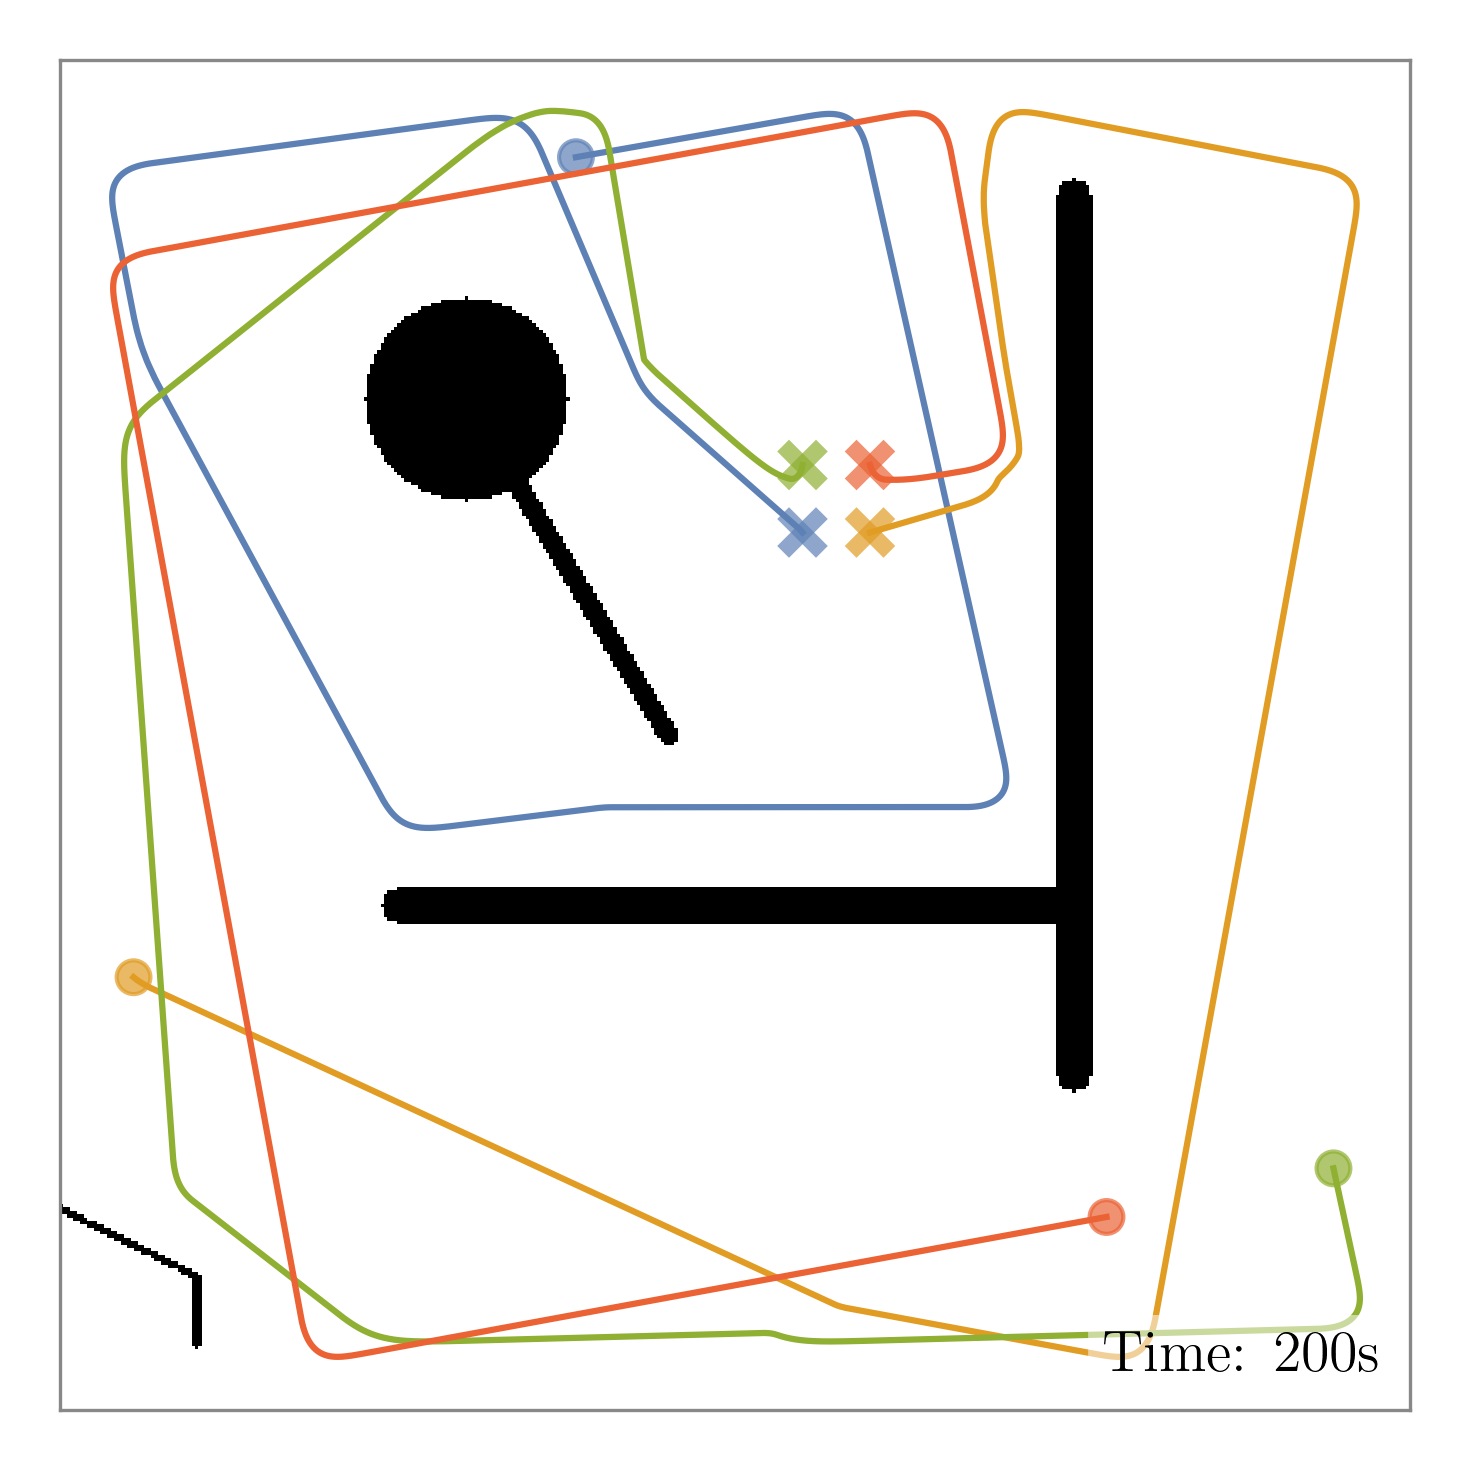
\includegraphics[width=\textwidth]{./figures/plots/paths/avoid-obstacles-paths-(after-200s).png}
    \end{subfigure}
    \begin{subfigure}[b]{\w}
        \centering
        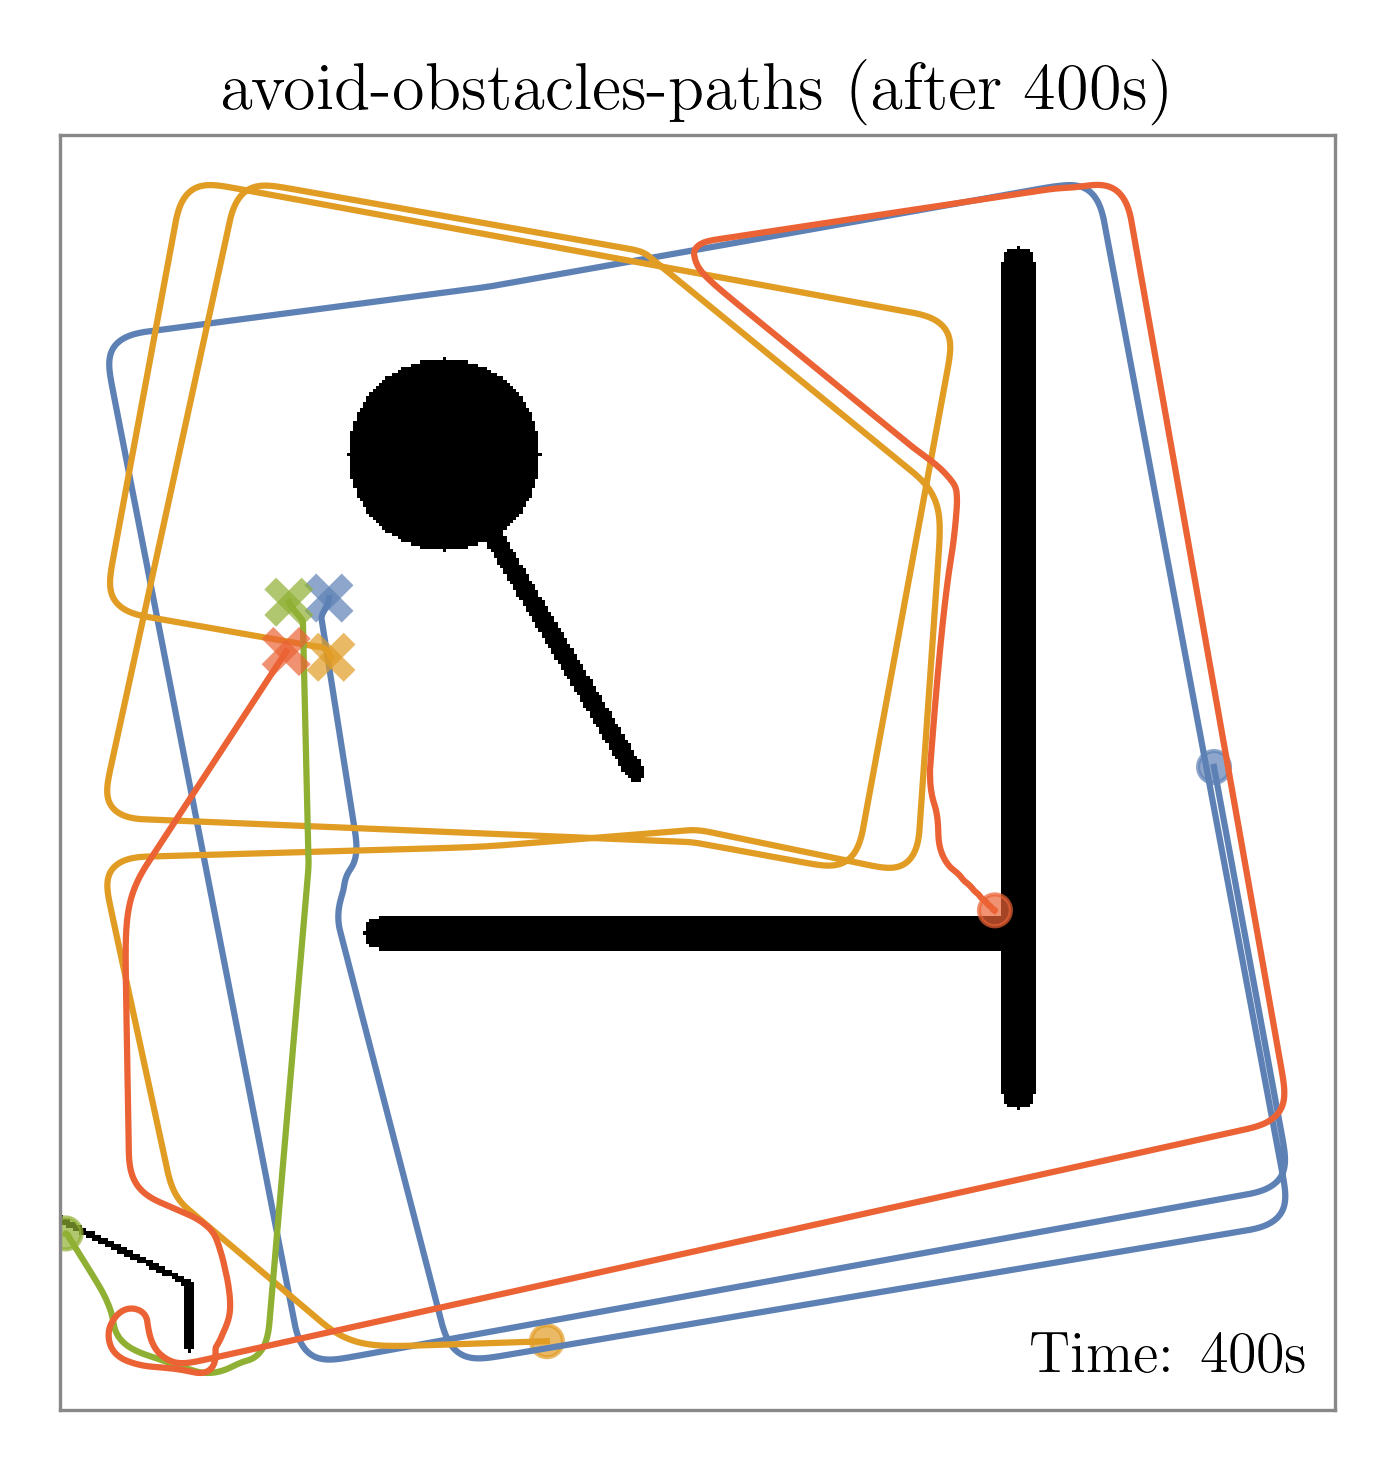
\includegraphics[width=\textwidth]{./figures/plots/paths/avoid-obstacles-paths-(after-400s).png}
    \end{subfigure}
    \begin{subfigure}[b]{\w}
        \centering
        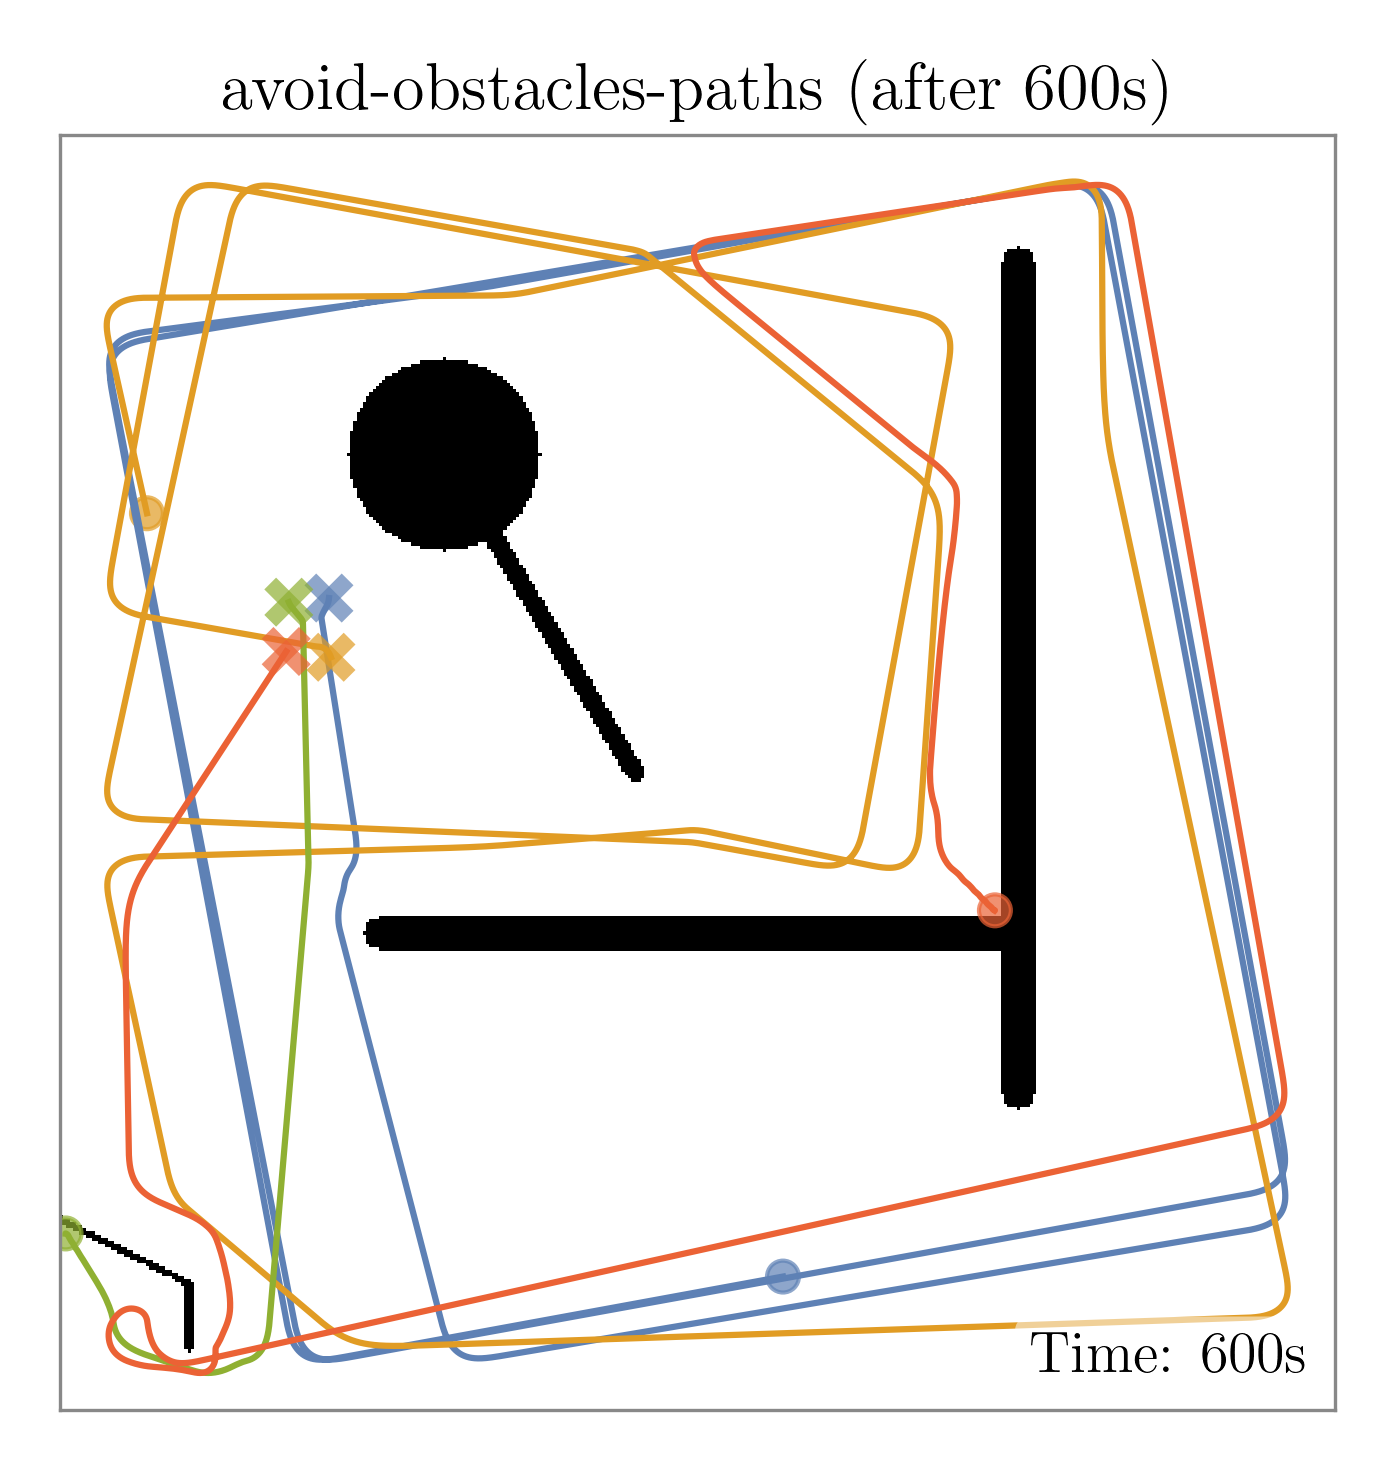
\includegraphics[width=\textwidth]{./figures/plots/paths/avoid-obstacles-paths-(after-600s).png}
    \end{subfigure}
    \caption{Paths of four robots running the obstacle avoidance algorithm in an example world simulated using \texttt{simple\_sim}. Crosses mark starting positions; circles indicate end positions.}
    \label{fig:roomba-paths}
\end{figure}

\subsection{Target Contributions}
Each robot maintains an internal state, which—combined with sensor input—drives its movement and exploration behavior. Conflicting objectives may arise; for instance, the robot may detect an unexplored area ahead but find its path blocked by an obstacle. One subsystem may suggest moving forward, while another recommends avoiding the obstacle.

To resolve this, each subsystem outputs a directional vector, or "target contribution," indicating its preferred movement. These vectors are then summed to produce a single target vector, which dictates the robot’s final motion. Subsystems can be weighted according to their importance—obstacle avoidance, for instance, is typically given higher priority. \Cref{fig:target-contributions} illustrates this principle.

\begin{figure}[H]
    \begin{center}
        \includegraphics[width=0.75\textwidth]{figures/target-contribtions.png}
    \end{center}
    \caption{Illustration of target vector calculation based on weighted subsystem contributions.}
    \label{fig:target-contributions}
\end{figure}


% TODO: Describe the idea, that different factors contribute to the target vector. The target vector is the sum over all contributions.
% TODO: Describe how we take gradients on a grid

\subsection{Search Grid}

Each robot maintains a "search grid," which acts as a heatmap representing the exploredness of each cell in the map. This grid is continuously updated using the robot’s own observations and messages received from other robots via the shared communication channel. Explored areas are considered "cold," while unexplored areas are "hot."\\

Assuming lossless communication, the search grids across robots should remain synchronized. Each robot computes a directional gradient from this heatmap at its current position, encouraging movement toward hotter (less explored) regions, as shown in \cref{fig:search-gradient-no-forward} and \cref{fig:search-gradient-forward}.

% TODO: Maybe not have this picture. But maybe nice to see without forward bias
\begin{figure}[H]
    \begin{center}
        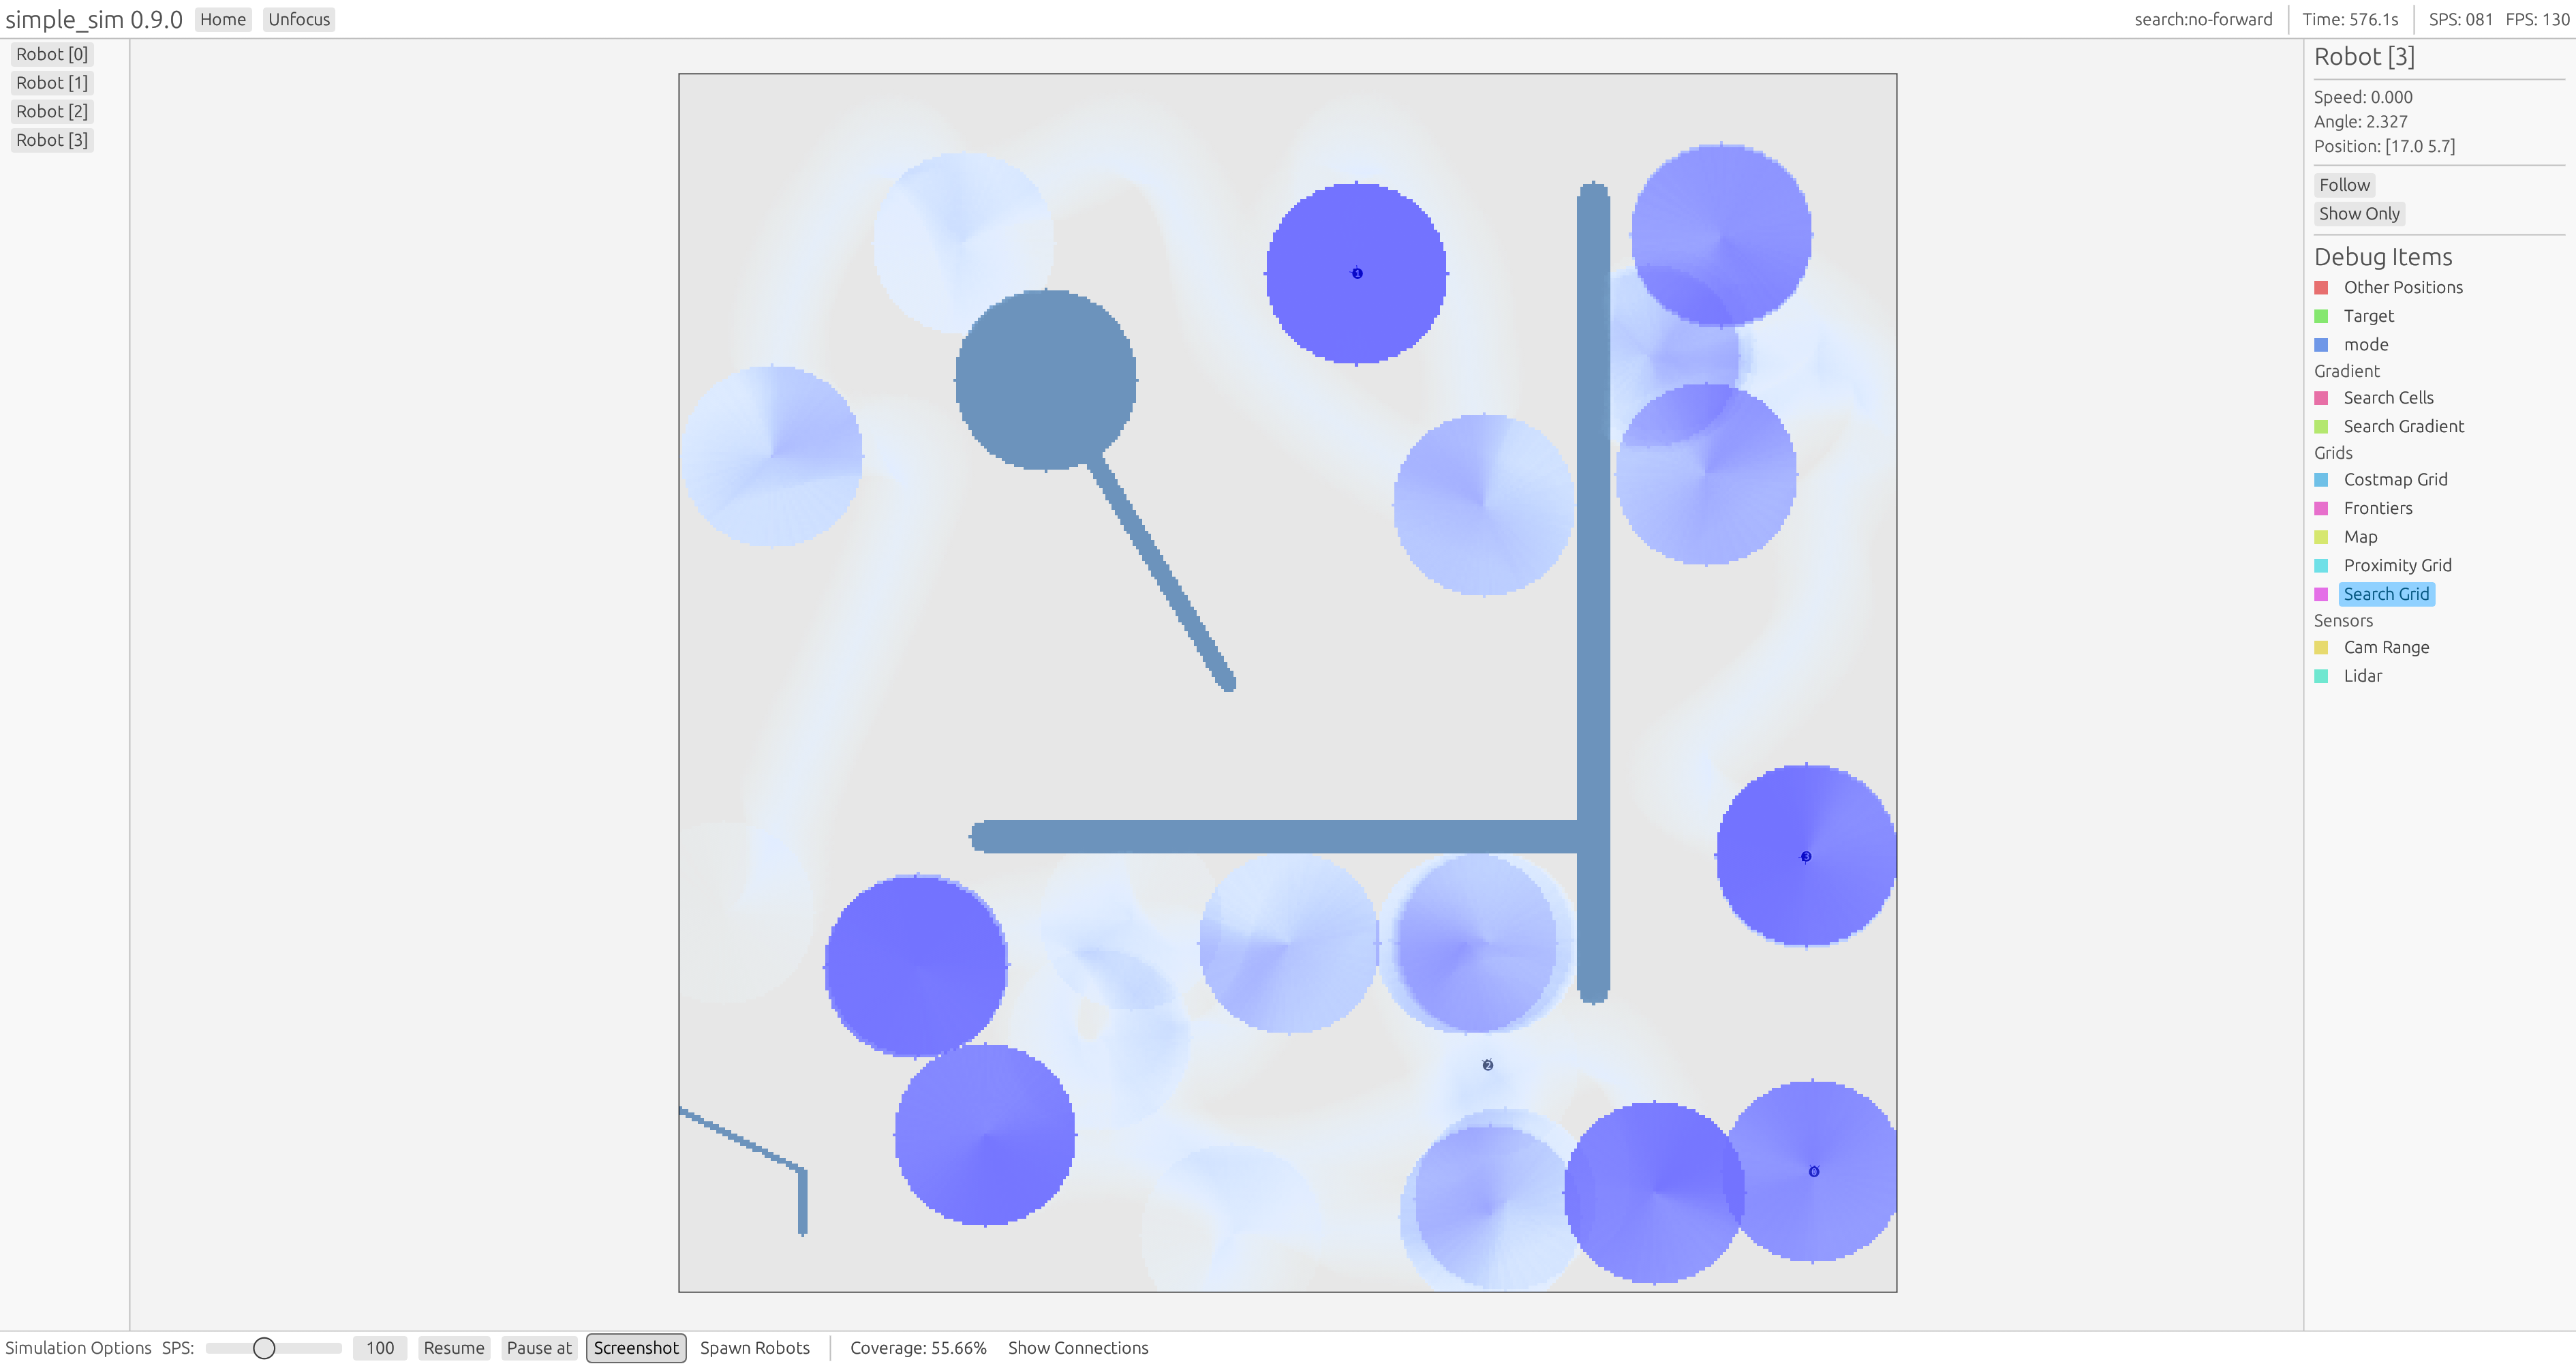
\includegraphics[width=0.85\textwidth]{./figures/screenshots/no-forward.png}
    \end{center}
    \caption{Gradient-based direction derived from the search grid without forward bias.}
    \label{fig:search-gradient-no-forward}
\end{figure}

\begin{figure}[H]
    \begin{center}
        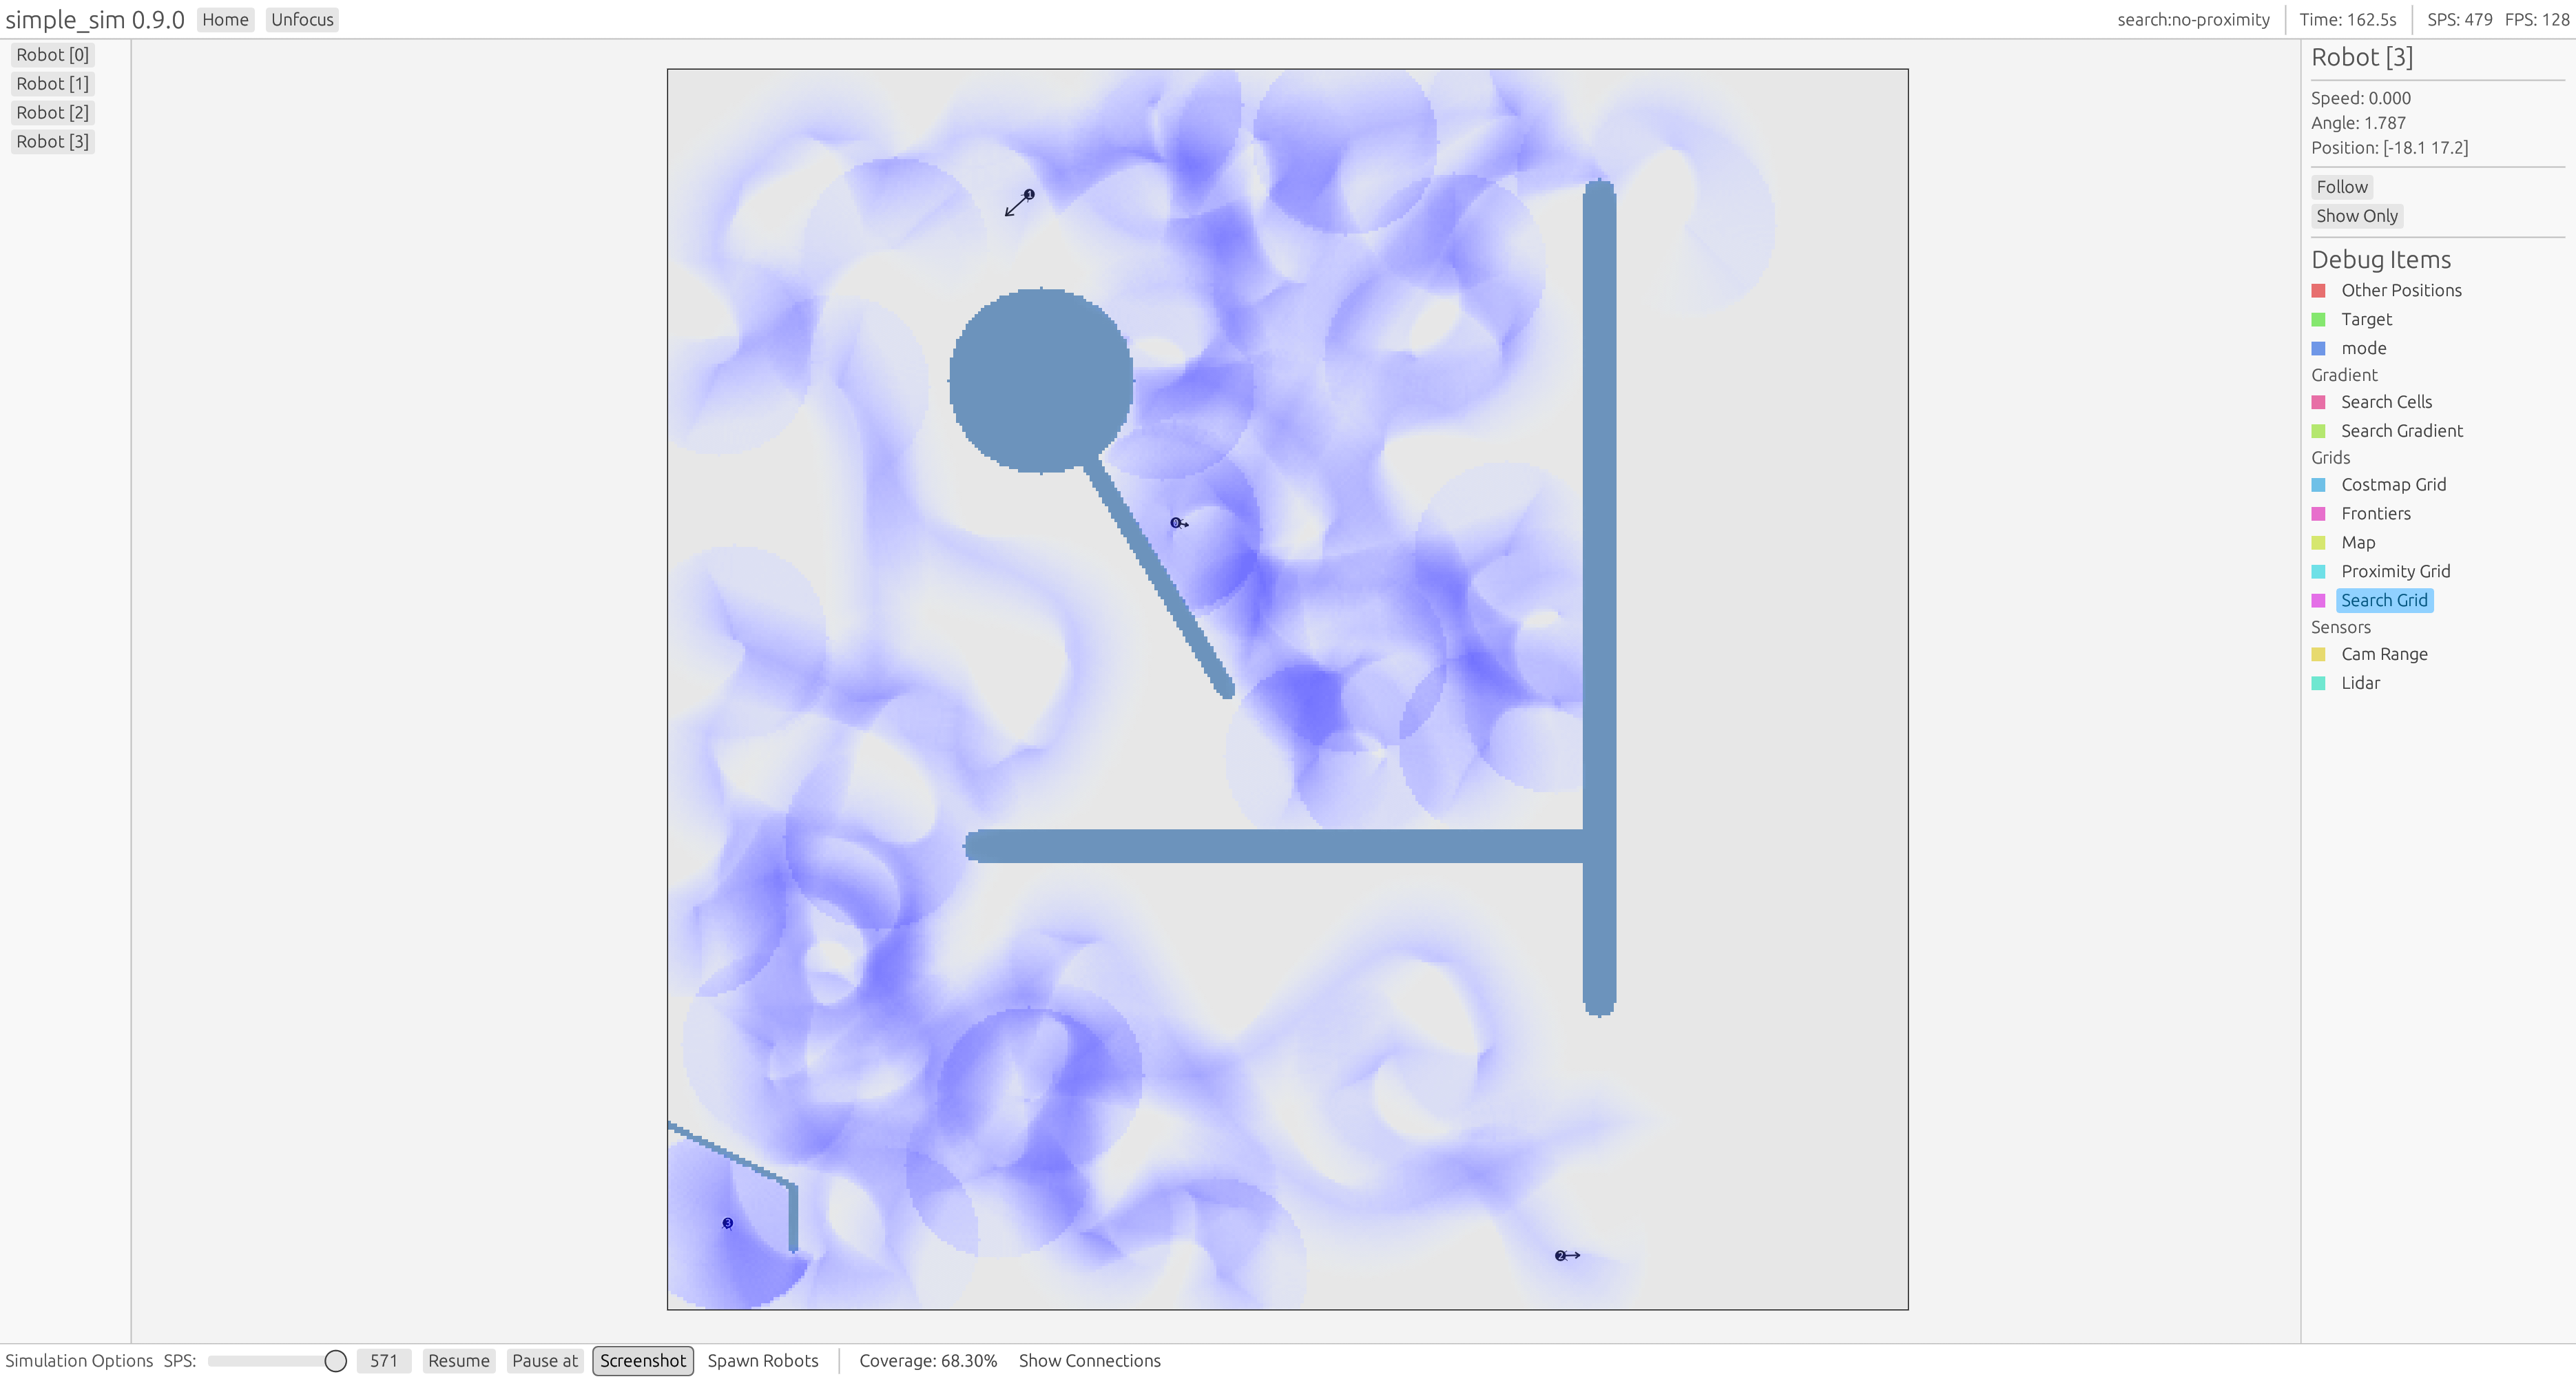
\includegraphics[width=0.85\textwidth]{./figures/screenshots/with-forward.png}
    \end{center}
    \caption{Gradient-based direction derived from the search grid with forward bias.}
    \label{fig:search-gradient-forward}
\end{figure}

In practice, computing the gradient involves several steps. First, the average heat under the robot ($H$) must be calculated. This is accomplished with the cells underneath the robot ($C_\mathrm{robot}$), as in \cref{eq:robot-heat}. $N$ is the number of cells in $C_\mathrm{robot}$.

\begin{equation}
\label{eq:robot-heat}
    H = \frac{1}{N} \sum_c^{C_\mathrm{robot}} \mathrm{heat}(c)
\end{equation}

Next, a vector $\mathbf{d}$ is computed from the robot's position $P$ to every grid cell within a specified radius ($C_\mathrm{r}$):

\begin{equation}
    \mathbf{d} = \mathrm{pos}(c) - P, \quad \forall c \in C_\mathrm{r}
\end{equation}

Each cell contributes to the final gradient based on the difference in heat and its proximity to the robot. The contribution fades linearly with distance, resulting in the following expression:

\begin{equation}
    \nabla = \sum_c^{C_\mathrm{r}} \;
    \underbracket{\; \mathbf{d}/\norm{\mathbf{d}}      \;}_\text{\makebox[0pt]{Direction}} \cdot
    \underbracket{\; \big(\mathrm{heat}(c) - H\big)    \;}_\text{Heat Diff.} \cdot
    \underbracket{\; \big(1 - \norm{\mathbf{d}}/r\big) \;}_\text{Nearness}
    \label{eq:fade-gradient}
\end{equation}

This formulation works well in open areas but may behave undesirably near map edges. Since cells outside the map have no heat value, the gradient can incorrectly point toward the map boundary if surrounding cells are colder than the current position. 
% \Cref{fig:edge-gradient} illustrates this issue.

% TODO: Comment out for now, I think it makes sense without needing a picture
% \begin{figure}[h]
%     \begin{center}
%         \includegraphics[width=0.45\textwidth]{./figures/edge-gradient.png}
%     \end{center}
%     \caption{Incorrect gradient pointing toward the edge of the map.}
%     \label{fig:edge-gradient}
% \end{figure}

To address this, only positive heat differences are considered in the gradient calculation. In practice, this means that the gradient points towards the "hottest" direction, but not necessarily away from the "coldest" direction.
\begin{equation}
\label{eq:robot-gradient}
    \nabla = \sum_c^{C_\mathrm{r}}
    \begin{cases}
        \mathbf{d}/\norm{\mathbf{d}}      \; \cdot
        \big(\mathrm{heat}(c) - H\big)    \; \cdot
        \big(1 - \norm{\mathbf{d}}/r\big) \; \quad &\text{if } \mathrm{heat}(c) > H
        \\
        0, \quad &\text{otherwise}
    \end{cases}
\end{equation}

This modification prevents attraction toward map boundaries and ensures the robot continues to seek out unexplored areas. Cells occluded by obstacles are excluded from this computation.
% \Cref{fig:search-no-proximity} shows robot paths using this approach with a small forward bias added.

% \begin{figure}[h]
%     \begin{center}
%         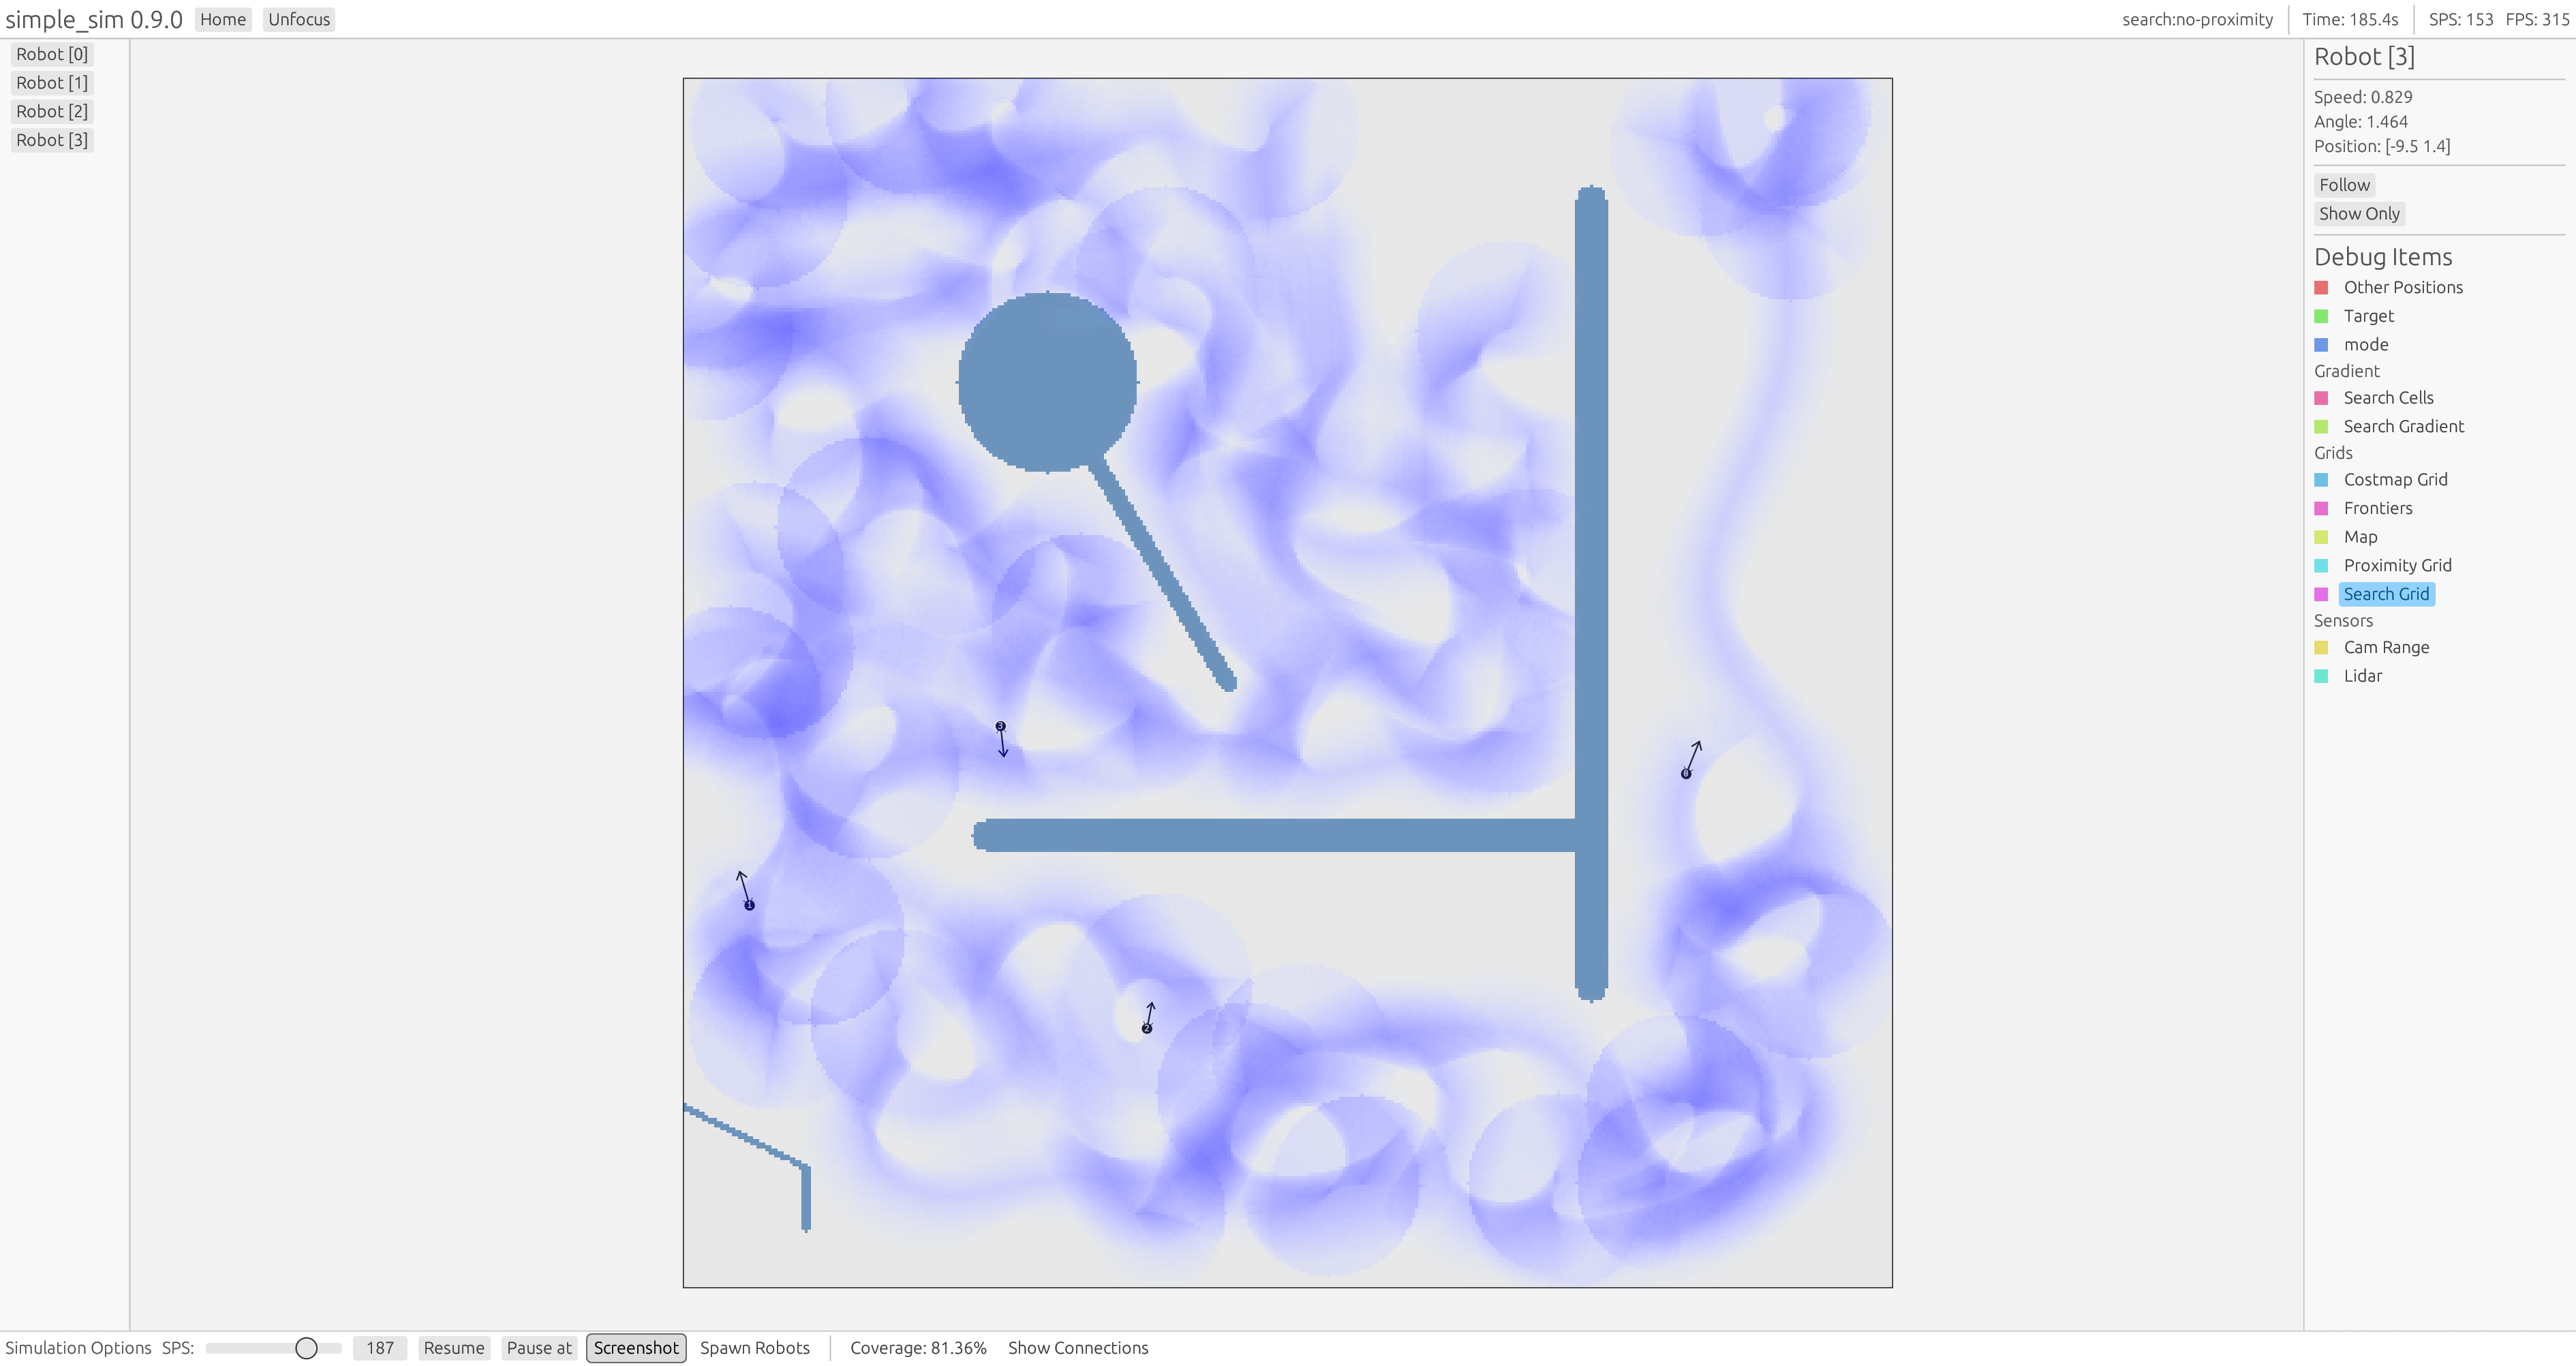
\includegraphics[width=0.85\textwidth]{./figures/screenshots/gradient.png}
%     \end{center}
%     \caption{Robot trajectories using gradient-based exploration.}
%     \label{fig:search-no-proximity}
% \end{figure}

\subsection{Proximity Grid}
To maintain network connectivity, robots must stay within communication range of each other. Each robot uses a "proximity grid" to estimate which areas of the map are within range of the main robot network (see \cref{fig:proximity-grid}).

\begin{figure}[h]
    \begin{center}
        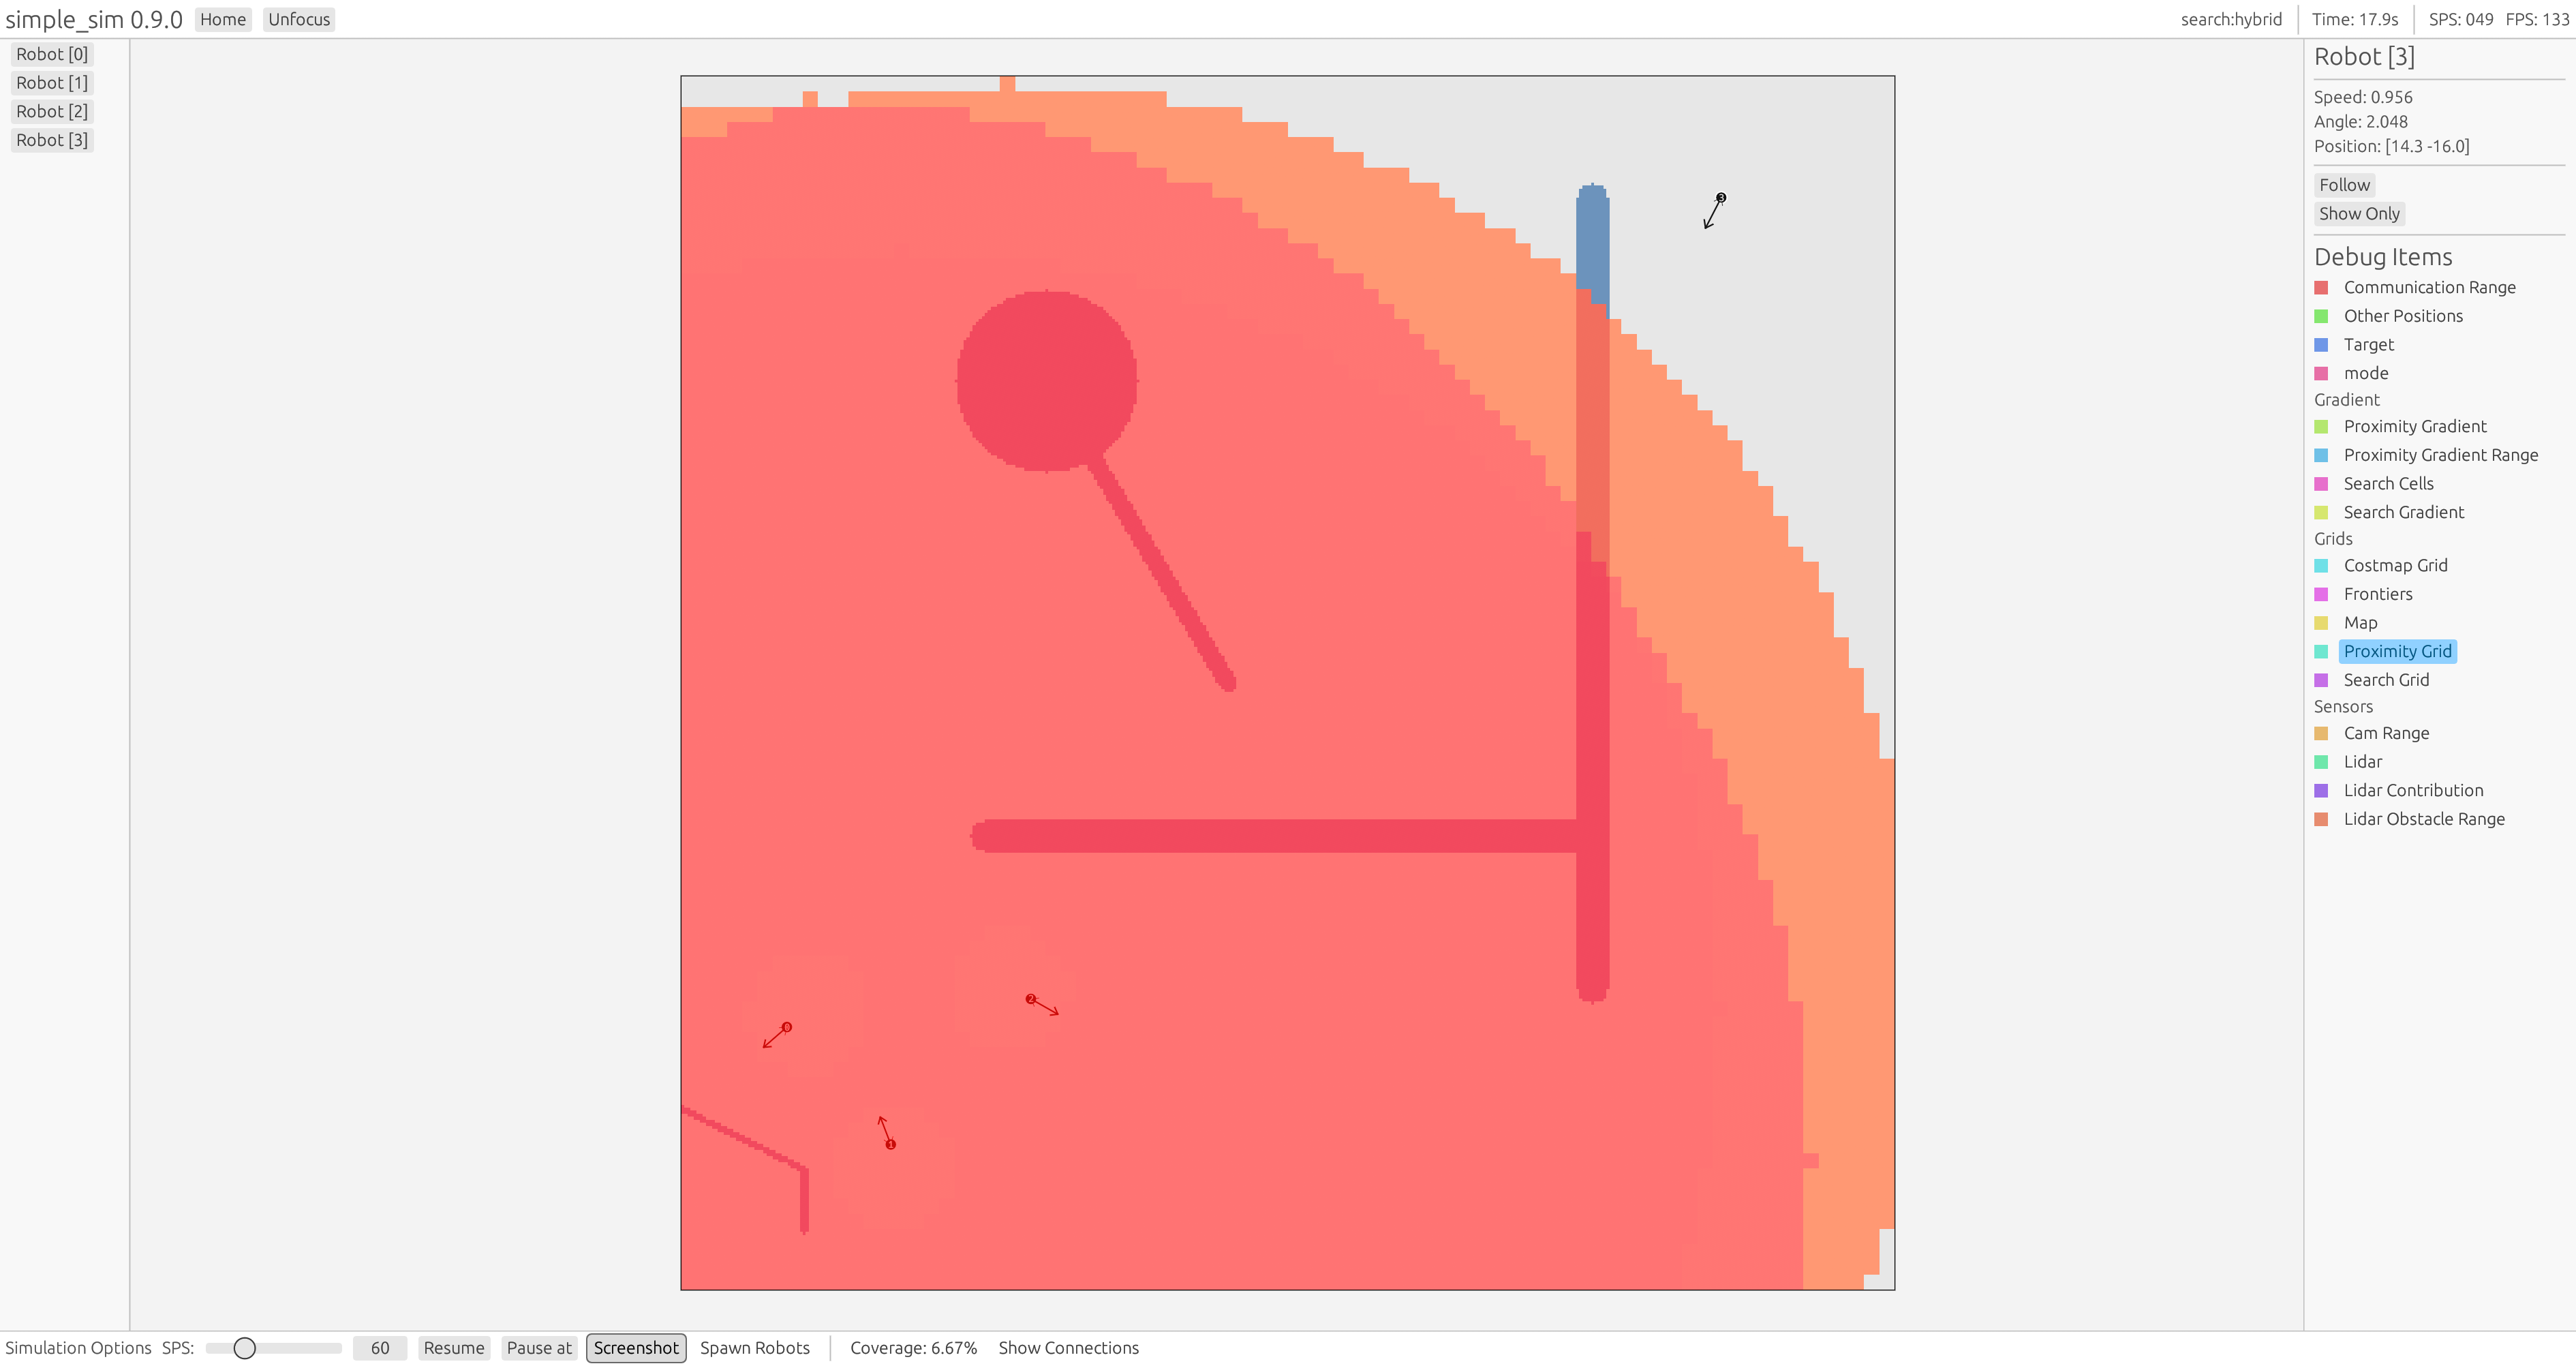
\includegraphics[width=0.85\textwidth]{figures/screenshots/proximity-gradient.png}
    \end{center}
    \caption{Proximity grid indicating areas connected to the main network.}
    \label{fig:proximity-grid}
\end{figure}

The proximity grid is computed by identifying the largest set of connected robots and "coloring" the reachable area from them. Tiles partially connected (e.g., by only one robot) are half-shaded to indicate weaker signal reliability. A gradient is computed over this grid and added as a weighted contribution to the robot’s overall target vector.

Importantly, each robot excludes itself when calculating the proximity grid. This ensures that if a robot is the sole link between two clusters, it will move toward the main network and draw disconnected robots with it.

This behavior is demonstrated in \cref{fig:proximity-pull}, where a single robot moves to reestablish group connectivity.

\def\w{0.329\textwidth}
\begin{figure}[h]
    \begin{center}
        \begin{subfigure}[b]{\w}
            \centering
            \includegraphics[width=\textwidth]{figures/proximity-pull1.png}
            \caption{Proximity grid for a \textcolor{red}{single-link} robot.}
            \label{fig:proximity-pull1}
        \end{subfigure}
        \begin{subfigure}[b]{\w}
            \centering
            \includegraphics[width=\textwidth]{figures/proximity-pull2.png}
            \caption{The robot moves toward the main network.}
            \label{fig:proximity-pull2}
        \end{subfigure}
        \begin{subfigure}[b]{\w}
            \centering
            \includegraphics[width=\textwidth]{figures/proximity-pull3.png}
            \caption{Stray robots are pulled back into the network.}
            \label{fig:proximity-pull3}
        \end{subfigure}
    \end{center}
    \caption{Example of a \textcolor{red}{single-link} robot reestablishing group connectivity.}
    \label{fig:proximity-pull}
\end{figure}


\subsection{Gradient Based-Algorithm}
The gradient-based algorithm calculates the robot's "target" vector using contributions from both the search and proximity grid gradients. However, when relying solely on these contributions, the resulting target vector often points sideways or even backward. This behavior occurs because the robot continuously "cools" down the area in front of its camera's field of view, which leads to excessive turning and minimal forward progress.

To mitigate this, a small constant forward vector is added to the total target vector to maintain movement and promote map coverage. \Cref{fig:gradient-paths} illustrates the paths of four robots executing this behavior.

\def\w{0.329\textwidth}
\begin{figure}[H]
    \centering
    \begin{subfigure}[b]{\w}
        \centering
        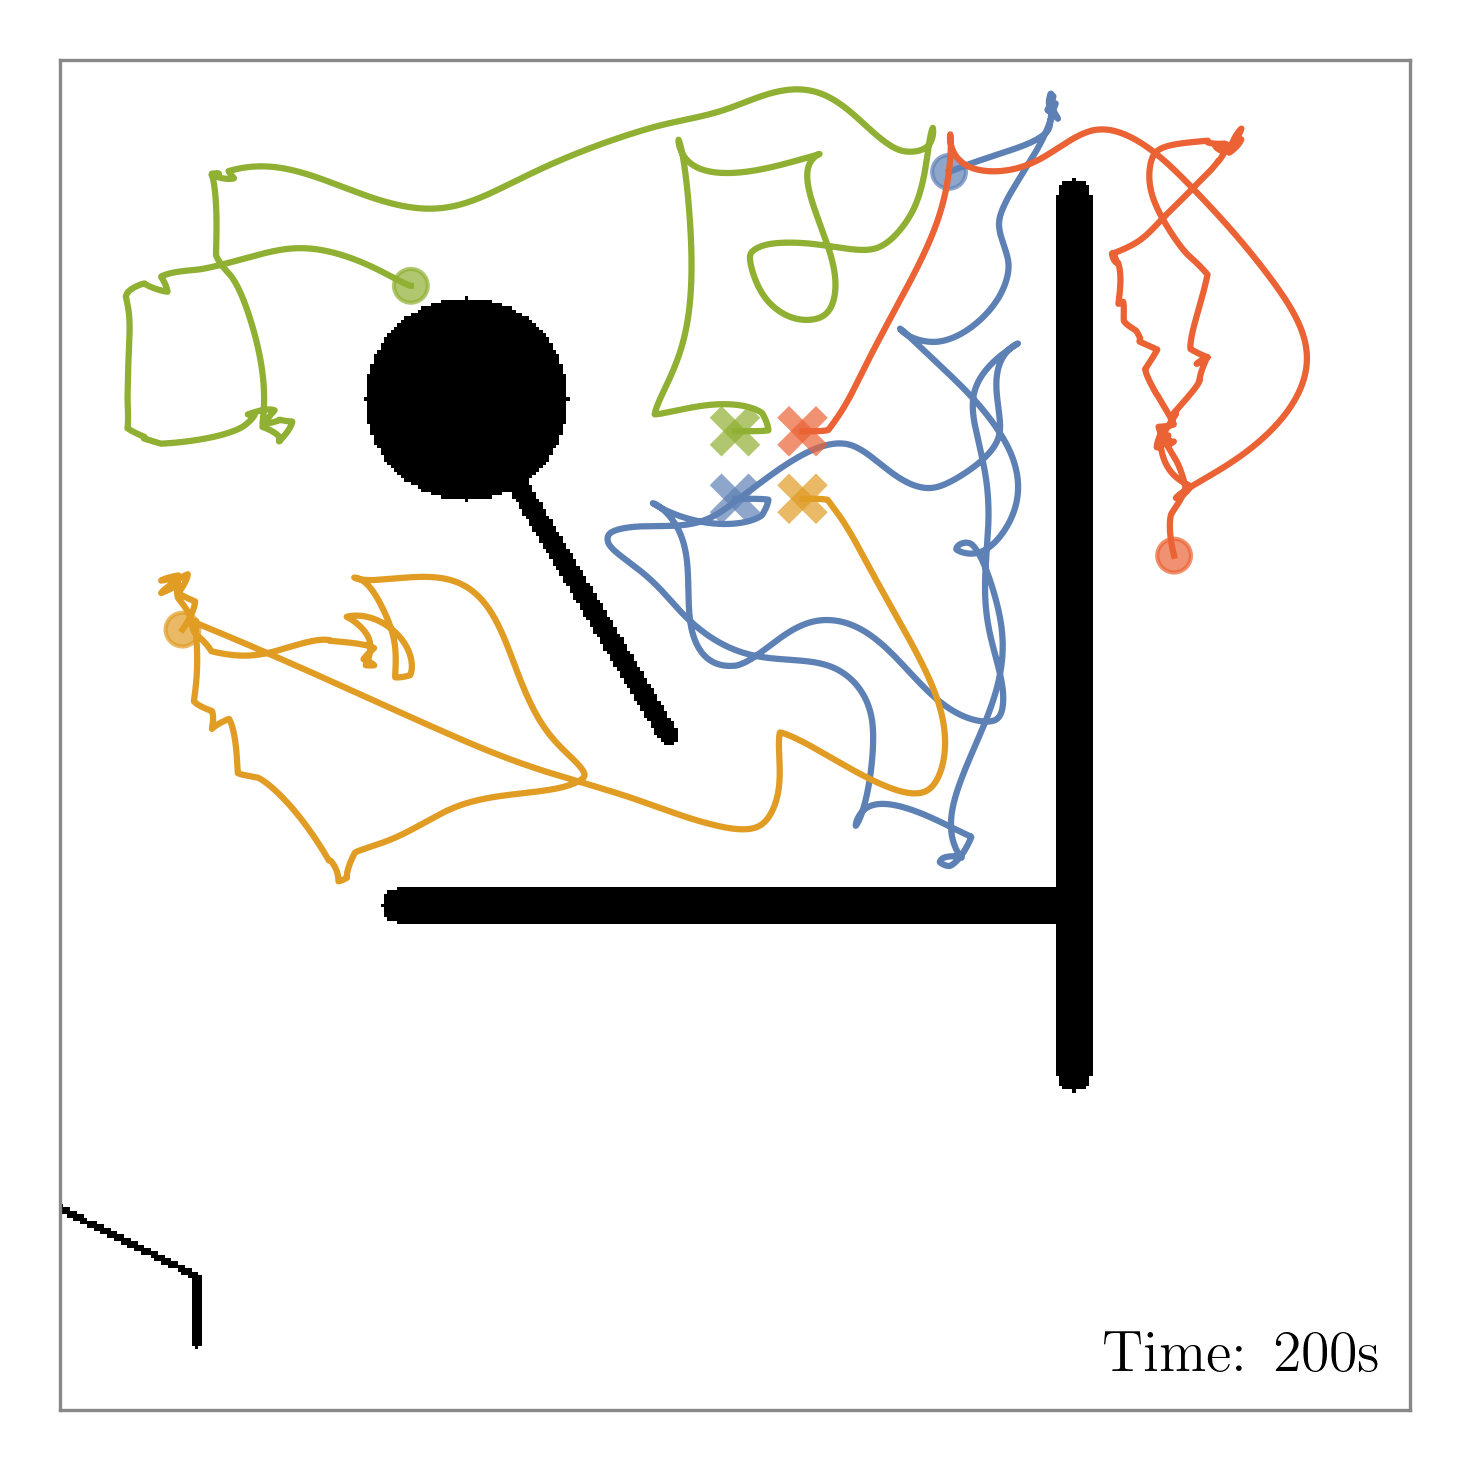
\includegraphics[width=\textwidth]{./figures/plots/paths/search:gradient-paths-(after-200s).png}
    \end{subfigure}
    \begin{subfigure}[b]{\w}
        \centering
        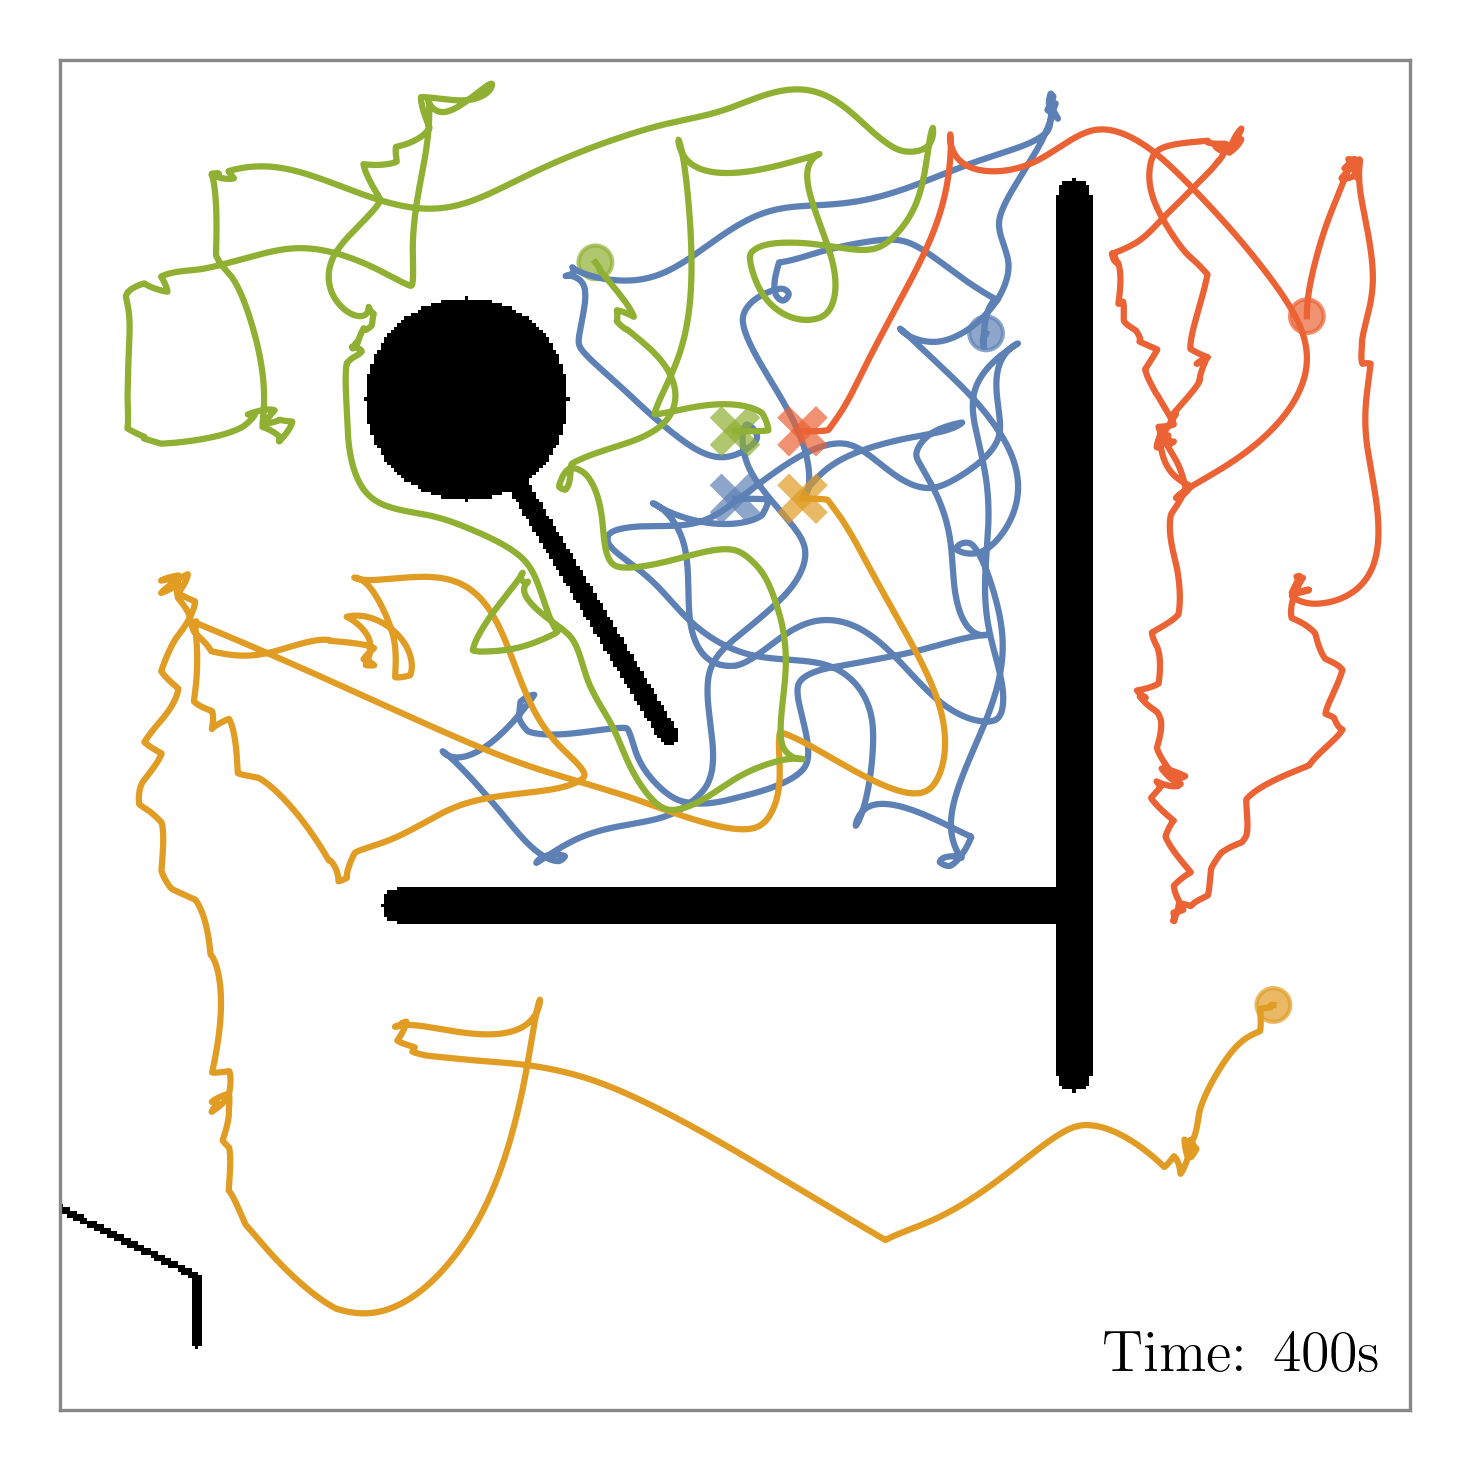
\includegraphics[width=\textwidth]{./figures/plots/paths/search:gradient-paths-(after-400s).png}
    \end{subfigure}
    \begin{subfigure}[b]{\w}
        \centering
        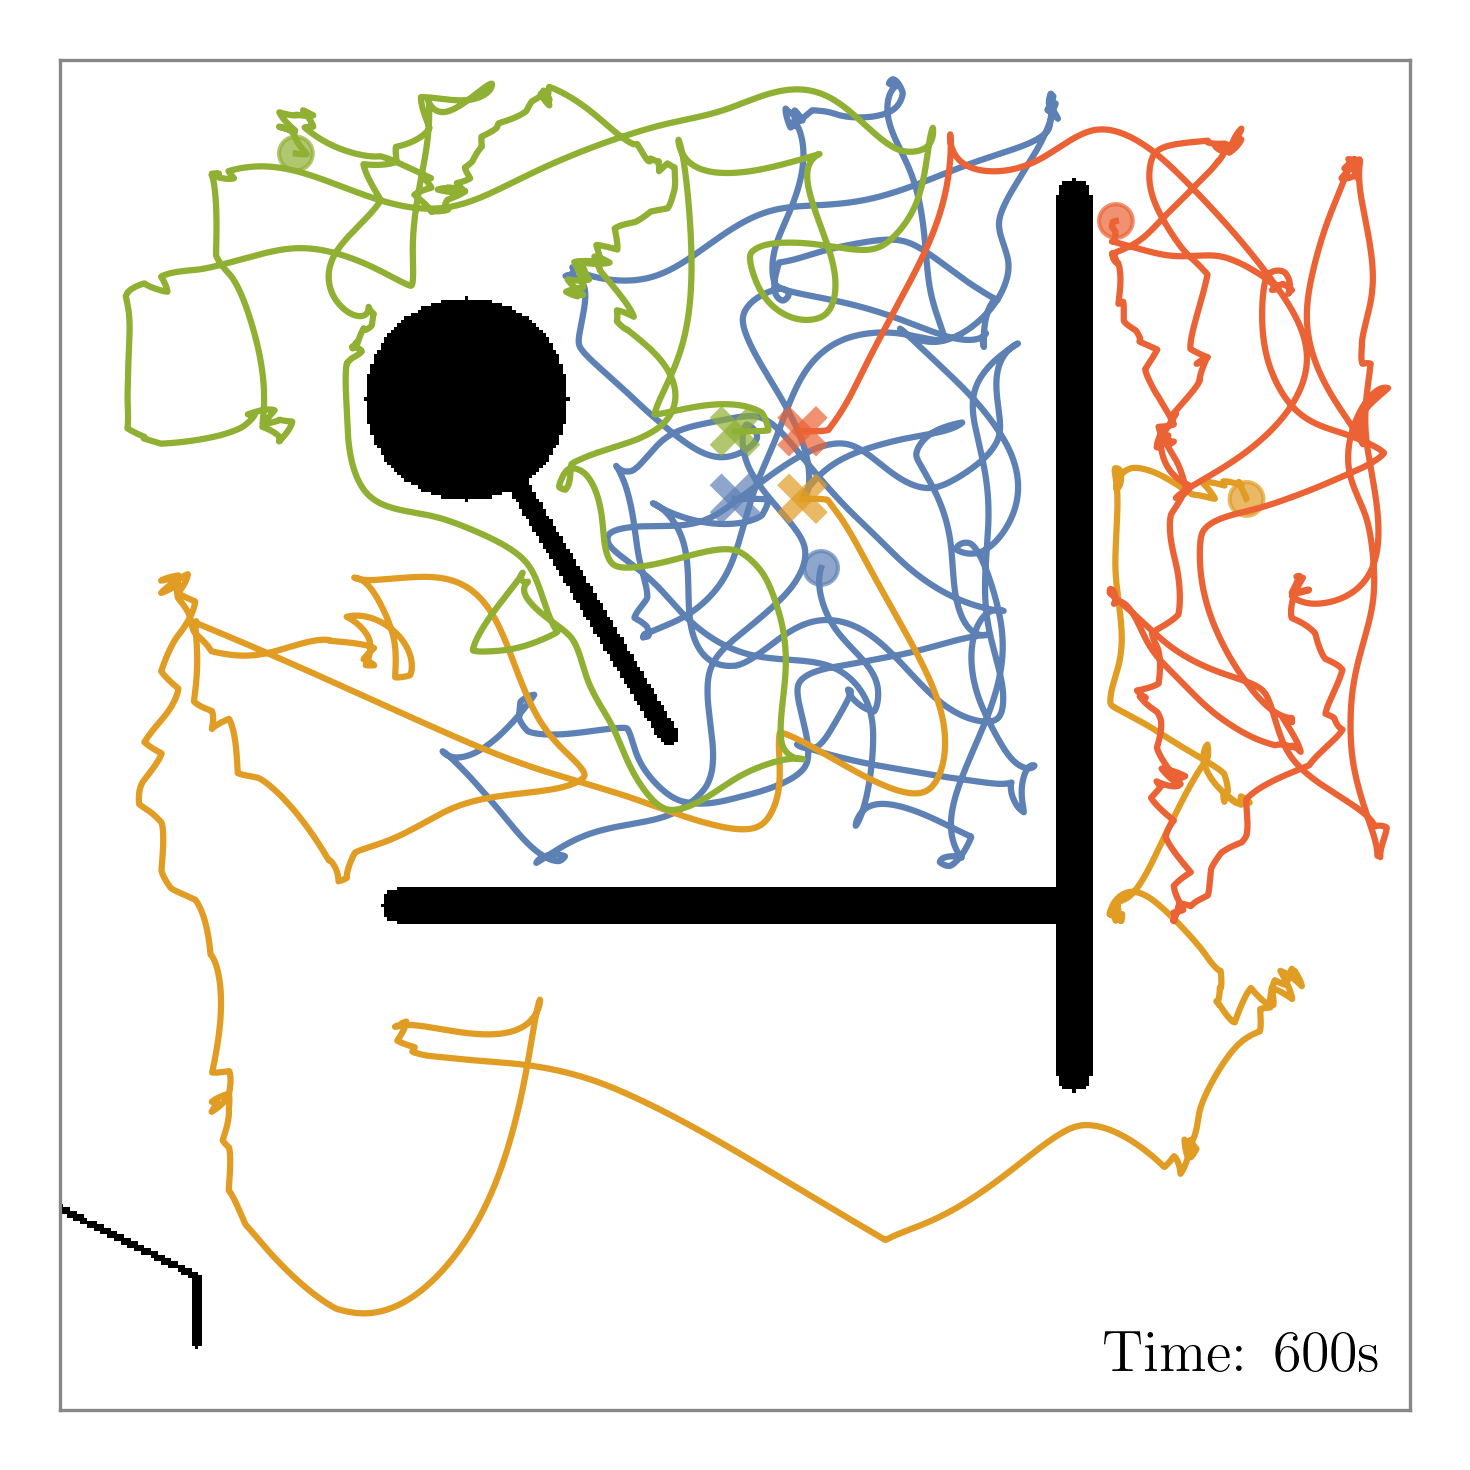
\includegraphics[width=\textwidth]{./figures/plots/paths/search:gradient-paths-(after-600s).png}
    \end{subfigure}
    \caption{Paths of four robots running the gradient-based algorithm in an example world simulated using \texttt{simple\_sim}. Crosses mark starting positions; circles indicate end positions.}
    \label{fig:gradient-paths}
\end{figure}

The robots explore the environment effectively but tend to linger in already explored regions. This behavior may result from the limited range used when calculating the search gradient. Additionally, robots exhibit more erratic paths when the gradient magnitude becomes small. In general, robots switch between smooth trajectories in unexplored areas and jagged paths when trapped in previously covered regions. To improve coverage, mechanisms that encourage movement toward globally unexplored areas would be beneficial.

\subsection{Global Planner}

When the search gradient fails to provide a clear direction—i.e., when the robot lacks a local preference—a global planner is used to move the robot to a more promising unexplored region.

% TODO: Mention something about performance later
% In cases, where computational resources are ample, the robot can rely entirely on path planning for navigation.

The global planner operates according to the following procedure:

\begin{enumerate}
  \item Generate a costmap (\cref{sec:costmap}).
  \item Identify frontiers and group them into regions (\cref{sec:frontier_exploration}).
  \item Evaluate the frontiers and select a goal (\cref{sec:frontier_exploration}).
  \item Plan a path using either a straight line or the A* algorithm (\cref{sec:path_planning}).
  \item Follow the path until the goal is reached or the path is invalidated (\cref{sec:path_following}).
\end{enumerate}

\subsubsection{Costmap}
\label{sec:costmap}
The costmap is a grid-based representation of the environment with a resolution of $0.2\,\text{m}$. Each cell in the costmap is assigned one of three states:

\begin{itemize}
  \item \textbf{Searched:} Cells identified as covered in the search grid.
  \item \textbf{Unknown:} Cells not yet visited.
  \item \textbf{Obstacle:} Cells corresponding to known obstacles or other robots, inferred from recent LiDAR readings.
\end{itemize}

% TODO: Show cost map and example of a planned route
\subsubsection{Frontier Exploration}
\label{sec:frontier_exploration}
A frontier is defined as a boundary between explored and unexplored regions. These frontiers are discovered using a Breadth-First Search (BFS) starting from the robot's current position. This approach avoids a full costmap scan, thereby reducing computational overhead.

Detected frontier cells are grouped into regions and scored based on:

\begin{itemize}
  \item Frontier region size
  \item Distance to the robot.
  \item Required turn angle to face the frontier.
\end{itemize}

Frontiers must also meet a minimum obstacle clearance threshold to be considered valid.

\begin{figure}[H]
    \centering
    \begin{subfigure}[b]{0.45\textwidth}
        \centering
        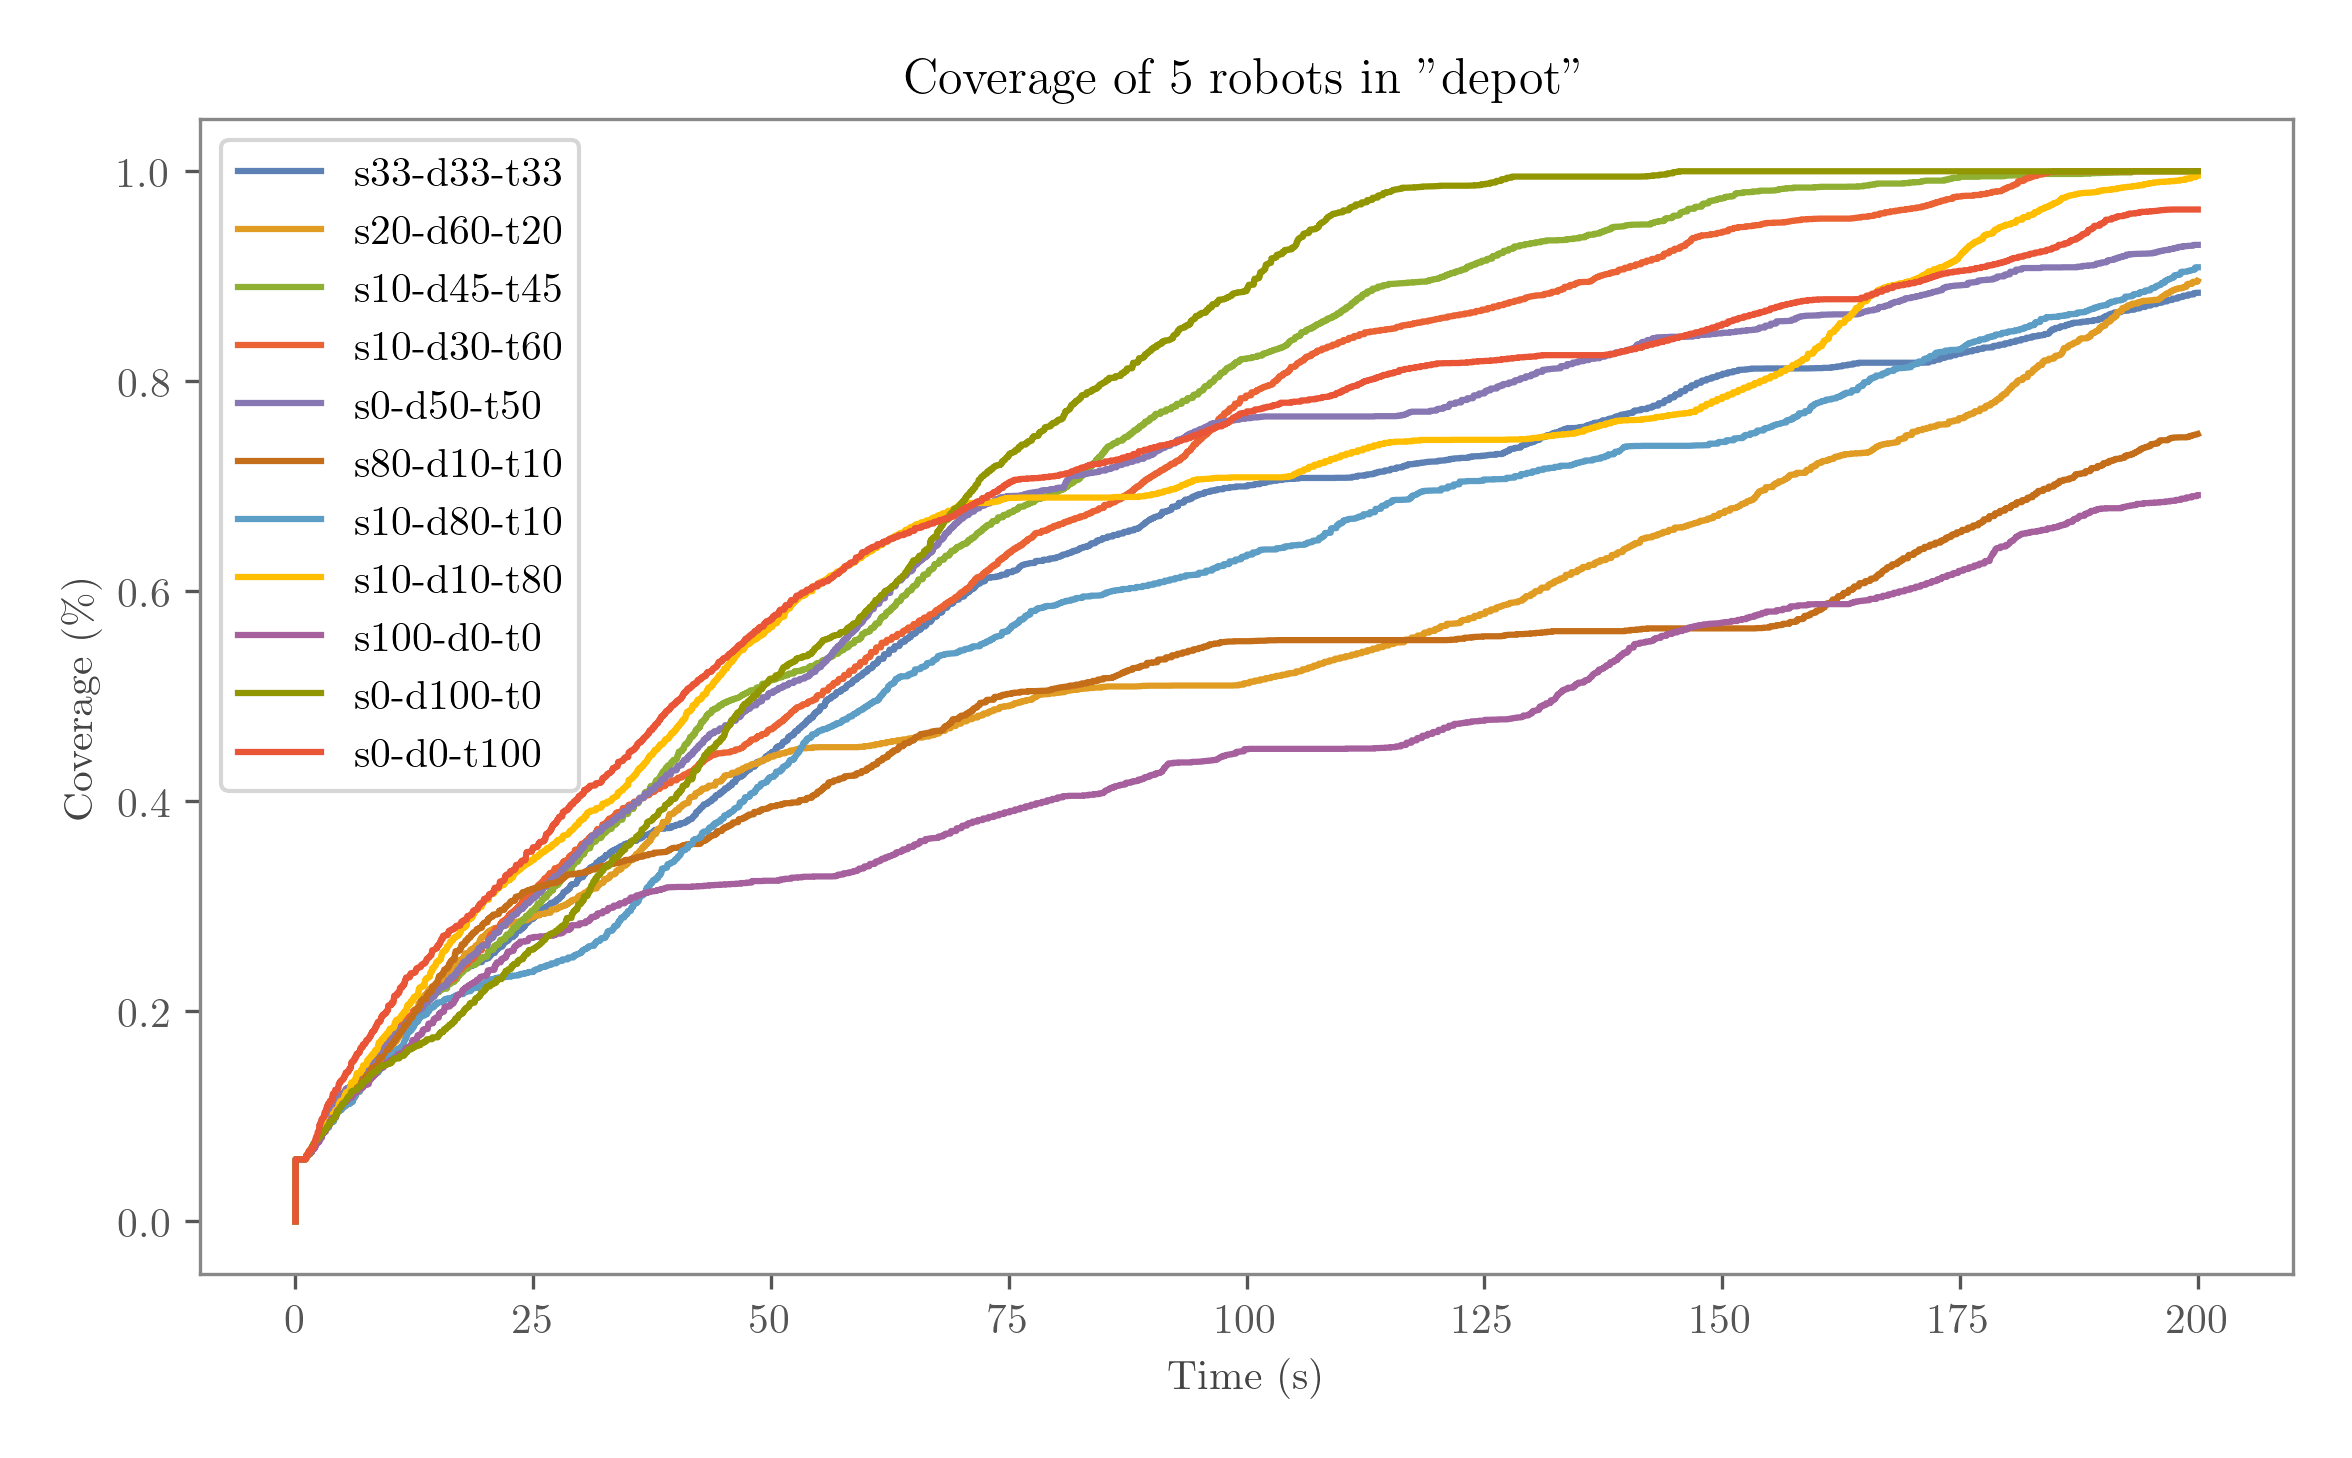
\includegraphics[width=\textwidth]{figures/frontier_eval_params_depot.png}
        \caption{Complex map}
    \end{subfigure}
    \hfill
    \begin{subfigure}[b]{0.45\textwidth}
        \centering
        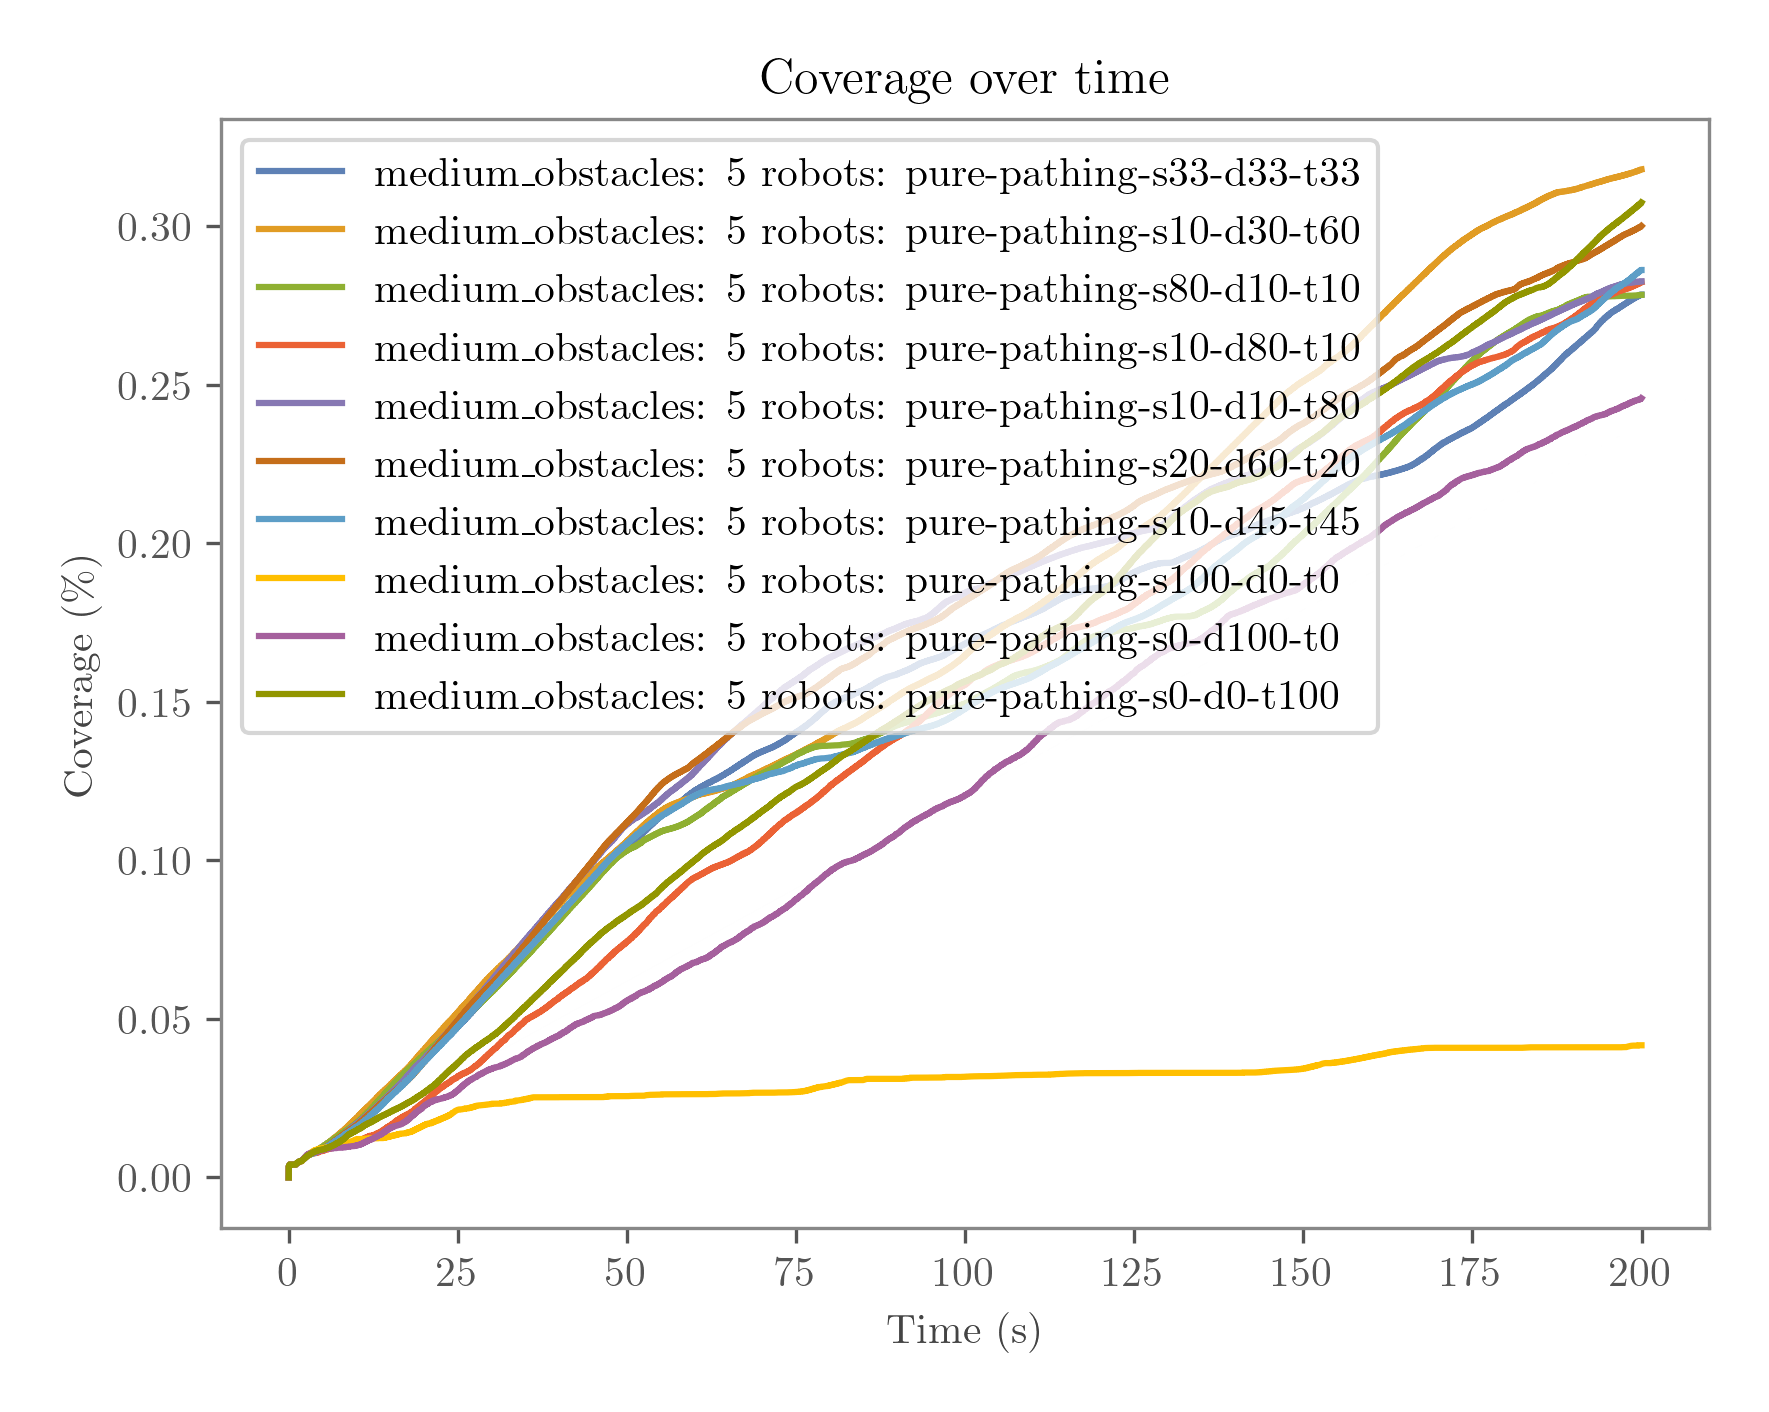
\includegraphics[width=\textwidth]{figures/frontier_eval_params_medium_obstacles.png}
        \caption{Simple map}
    \end{subfigure}
    \caption{Frontier evaluation parameters on two maps.}
    \label{fig:frontier-eval-params}
\end{figure}

These evaluations were conducted in two distinct environments. Line labels in \cref{fig:frontier-eval-params} indicate the parameter weightings used: \texttt{sXX} for frontier size, \texttt{dXX} for distance to the frontier, and \texttt{tXX} for the required turn angle. All tested configurations successfully achieved full map coverage; therefore, performance is evaluated based on coverage speed.

As shown in \cref{fig:frontier-eval-params}, configurations that prioritized distance and turn angle produced the fastest coverage. This outcome suggests that minimizing rotation allows for higher sustained forward velocity. In contrast, configurations that emphasized frontier size alone often resulted in inefficient behavior, such as long detours and frequent turning, which slowed down overall progress.

\subsubsection{Path Planning}
\label{sec:path_planning}
Once a goal is selected, the planner first attempts to use a direct straight-line path. If this path violates the clearance requirement, the A* algorithm is used instead.

A* explores cells using a heuristic that combines cumulative path cost and estimated distance to the goal. A min-heap is used to prioritize cells with the lowest estimated total cost. Only collision-free cells that meet clearance requirements are considered.

\subsubsection{Path Following}
\label{sec:path_following}
The robot follows the planned path as a sequence of waypoints. When it reaches a waypoint within a predefined threshold, that waypoint is marked as visited and removed from the path.

The path is continuously validated to account for dynamic changes in the environment. If a path segment becomes invalid, the robot continues toward the next waypoint while enabling LiDAR-based obstacle avoidance. If repeated validation fails, the robot replans. If replanning also fails, a new goal is selected.

To maintain communication, if a robot becomes disconnected from the swarm, it selects a new goal that helps it reconnect with the main network, using the proximity grid.

\subsection{Hybrid Algorithm}
The global planner enables a hybrid algorithm that combines both local and global strategies. As long as the local search gradient provides a sufficiently strong direction, the robot continues using the gradient-based method. When the gradient magnitude falls below a predefined threshold, the global planner is triggered to relocate the robot to an unexplored area.

\textcolor{red}{[Threshold definition or derivation to be inserted here.]}

The hybrid algorithm produces better spatial distribution and exploration efficiency. \Cref{fig:hybrid-paths} shows the resulting behavior, where solid lines represent gradient-based movement and dashed lines indicate global path-following.

\def\w{0.329\textwidth}
\begin{figure}[H]
    \centering
    \begin{subfigure}[b]{\w}
        \centering
        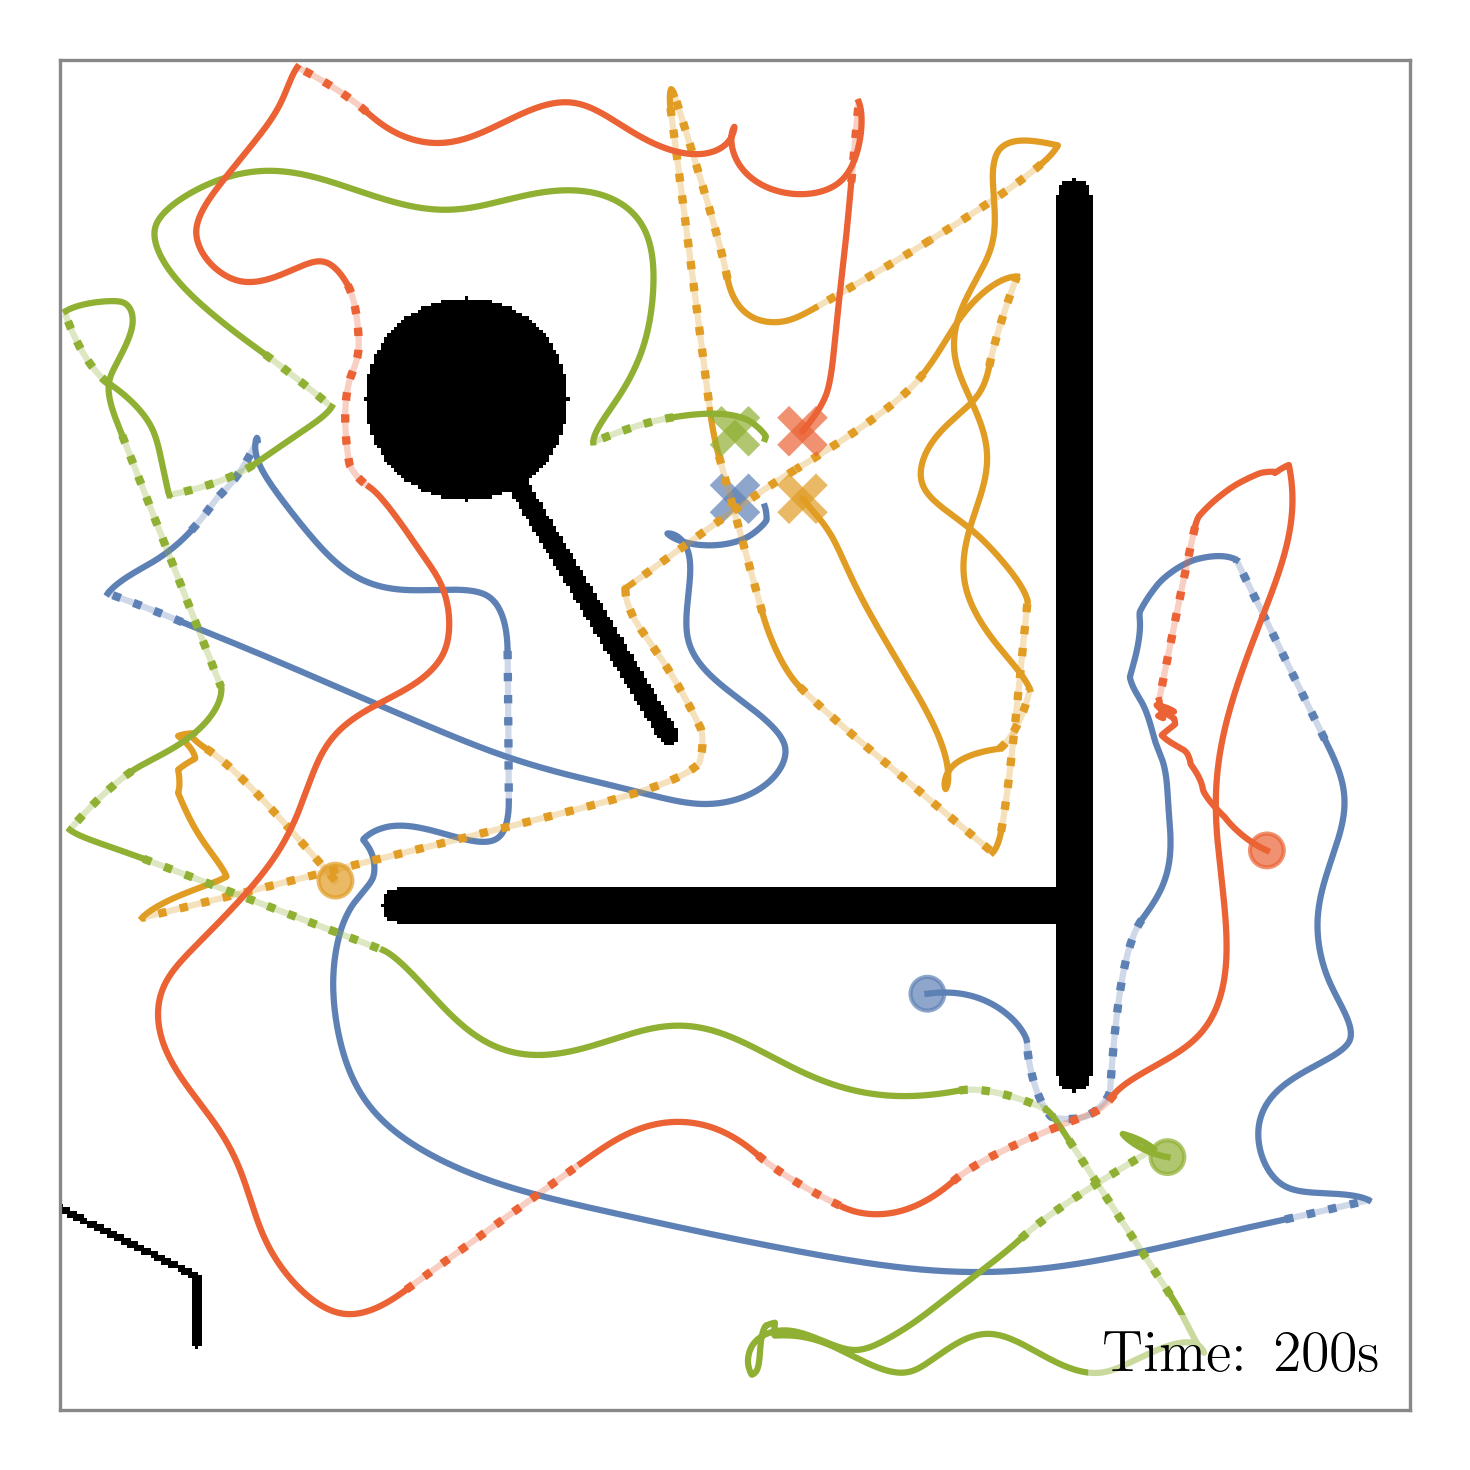
\includegraphics[width=\textwidth]{./figures/plots/paths/search:hybrid-paths-(after-200s).png}
    \end{subfigure}
    \begin{subfigure}[b]{\w}
        \centering
        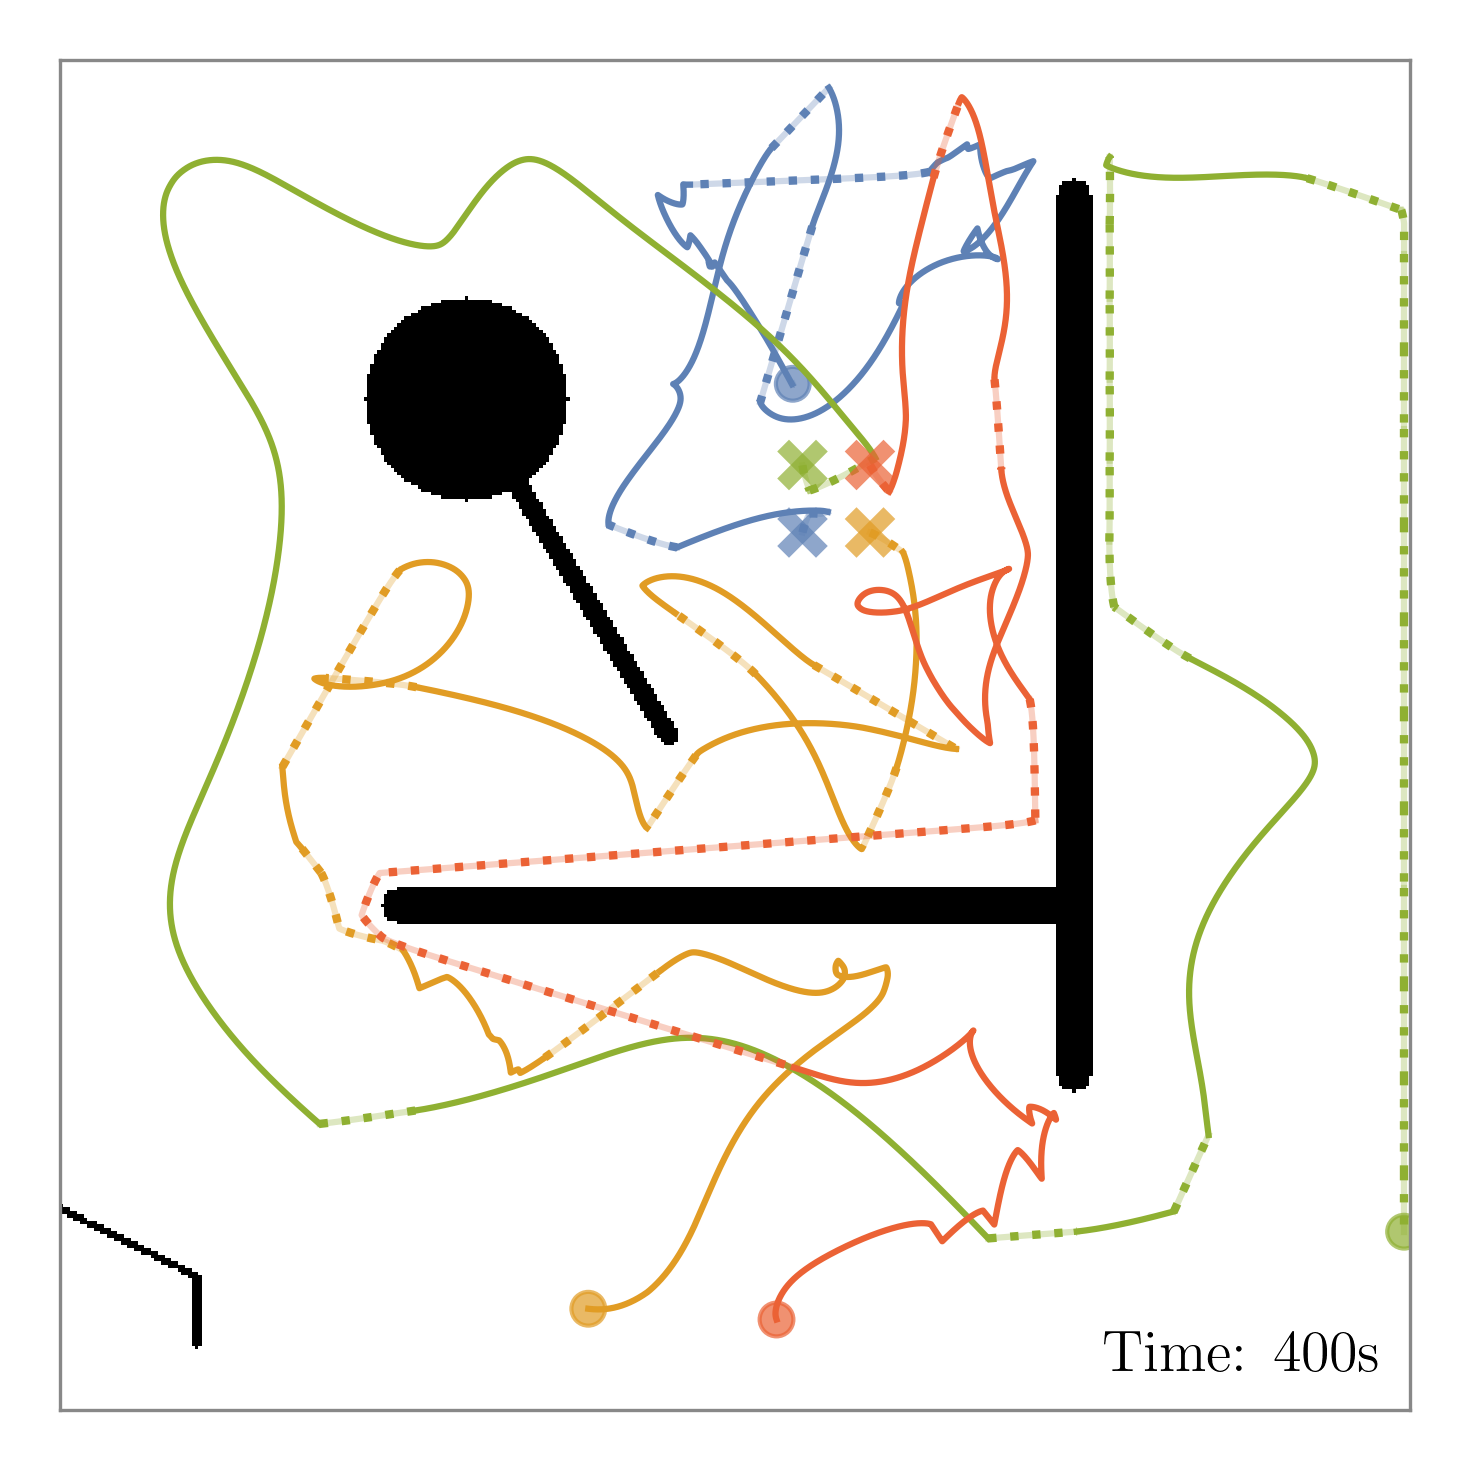
\includegraphics[width=\textwidth]{./figures/plots/paths/search:hybrid-paths-(after-400s).png}
    \end{subfigure}
    \begin{subfigure}[b]{\w}
        \centering
        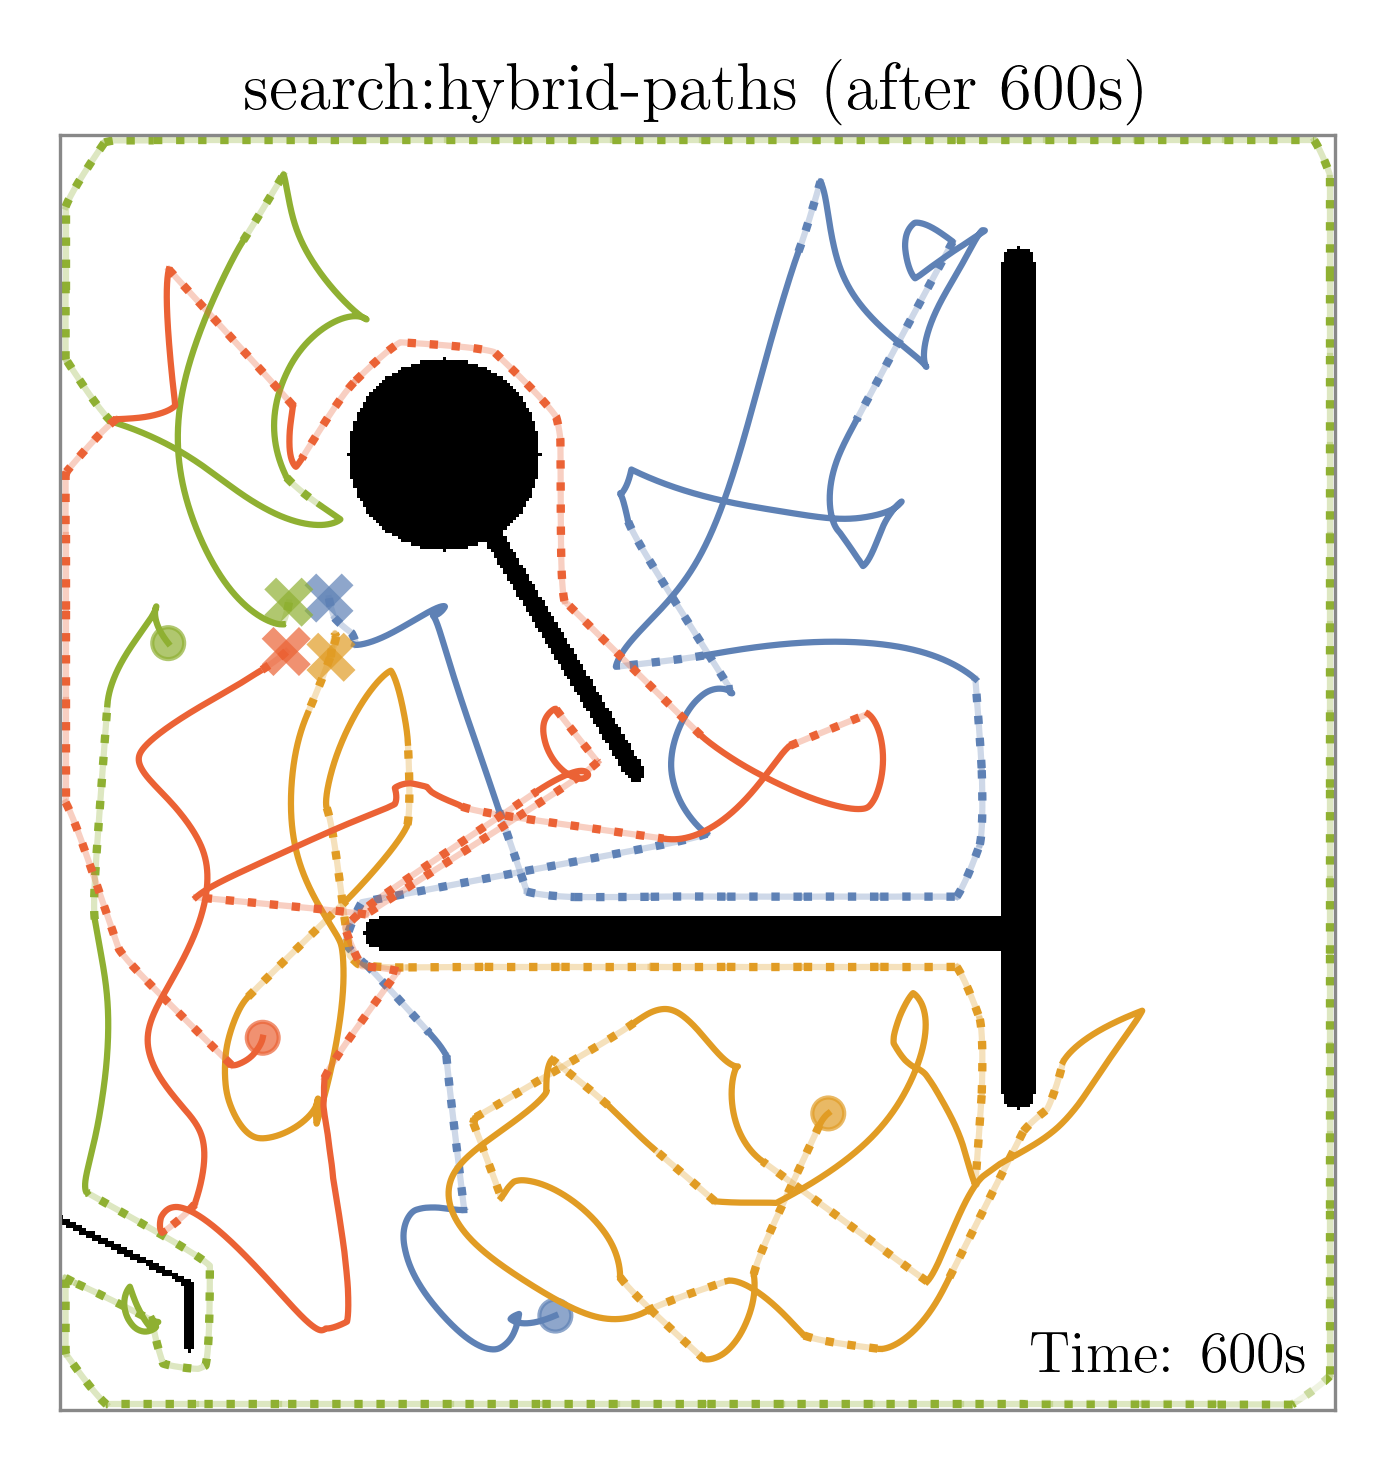
\includegraphics[width=\textwidth]{./figures/plots/paths/search:hybrid-paths-(after-600s).png}
    \end{subfigure}
    \caption{Paths of four robots running the hybrid algorithm in an example world simulated using \texttt{simple\_sim}. Solid lines indicate gradient-based motion; dashed lines indicate path-following; crosses mark starting positions; circles indicate end positions.}
    \label{fig:hybrid-paths}
\end{figure}

This approach results in faster and more complete coverage, with robots spending less time in already-explored regions compared to the pure gradient-based strategy.

\subsection{Pure Pathing Algorithm}
An alternative to the hybrid approach is to use the global planner exclusively. In this case, the robot continuously alternates between selecting a new goal and following the computed path.

\Cref{fig:pure-pathing-paths} shows example paths. As with the hybrid algorithm, the trajectories are smooth and consistent, with little aimless wandering.

% TODO: Fix broken paths
\def\w{0.329\textwidth}
\begin{figure}[H]
    \centering
    \begin{subfigure}[b]{\w}
        \centering
        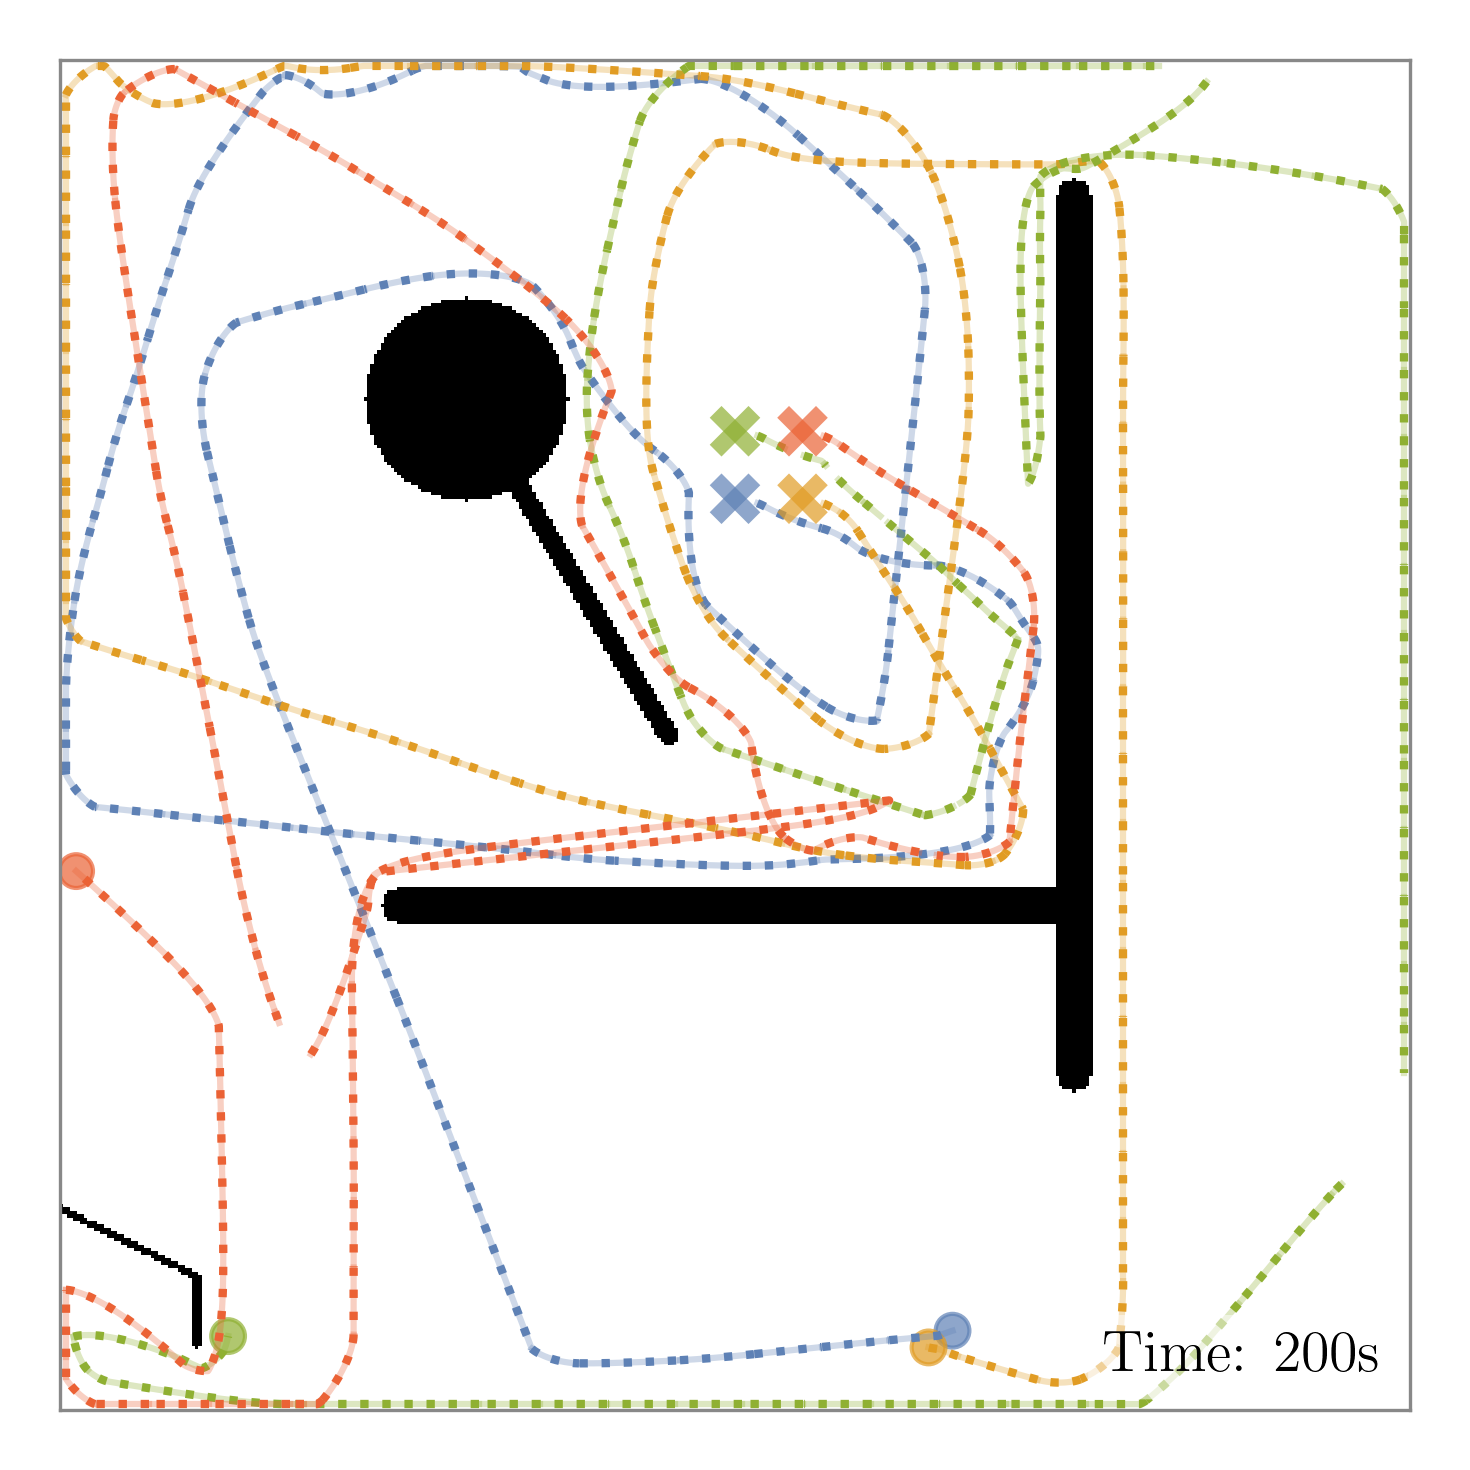
\includegraphics[width=\textwidth]{./figures/plots/paths/search:pathing-paths-(after-200s).png}
    \end{subfigure}
    \begin{subfigure}[b]{\w}
        \centering
        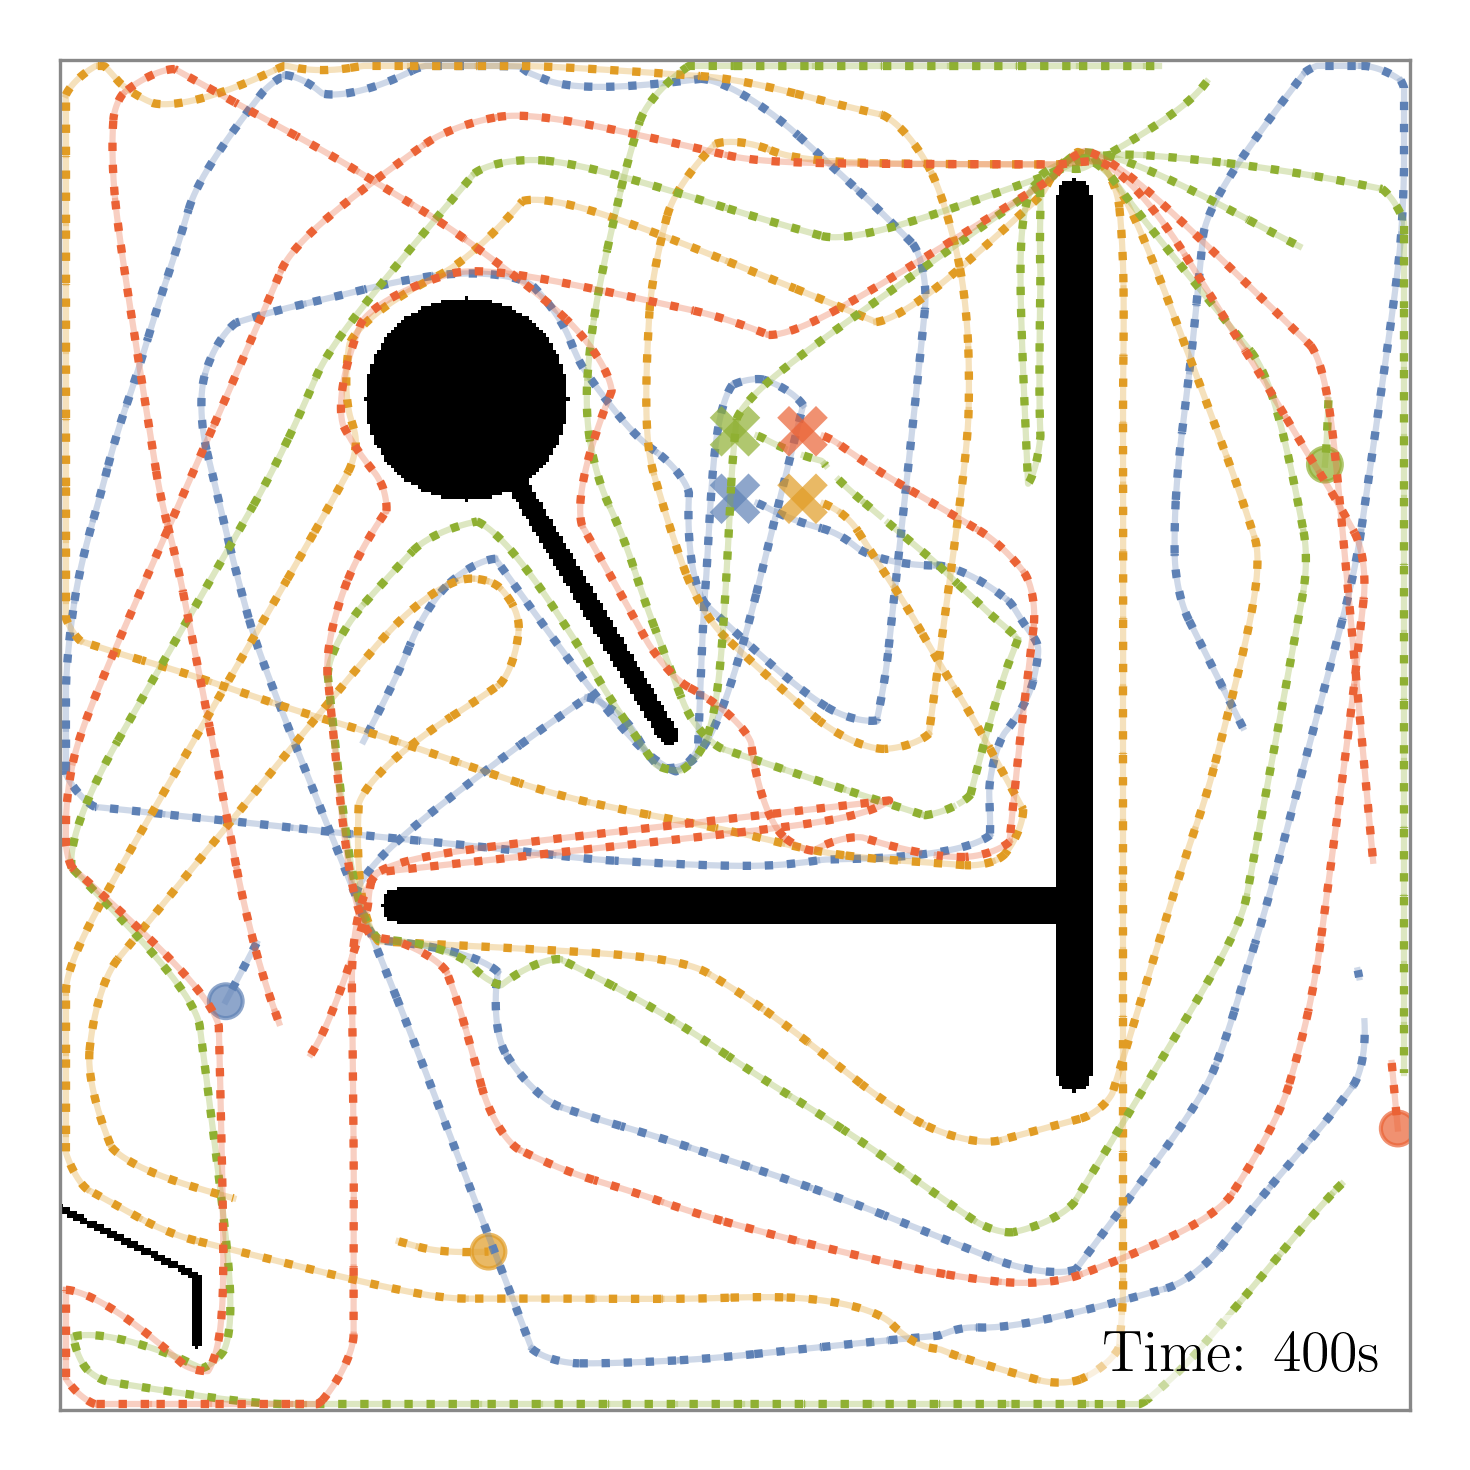
\includegraphics[width=\textwidth]{./figures/plots/paths/search:pathing-paths-(after-400s).png}
    \end{subfigure}
    \begin{subfigure}[b]{\w}
        \centering
        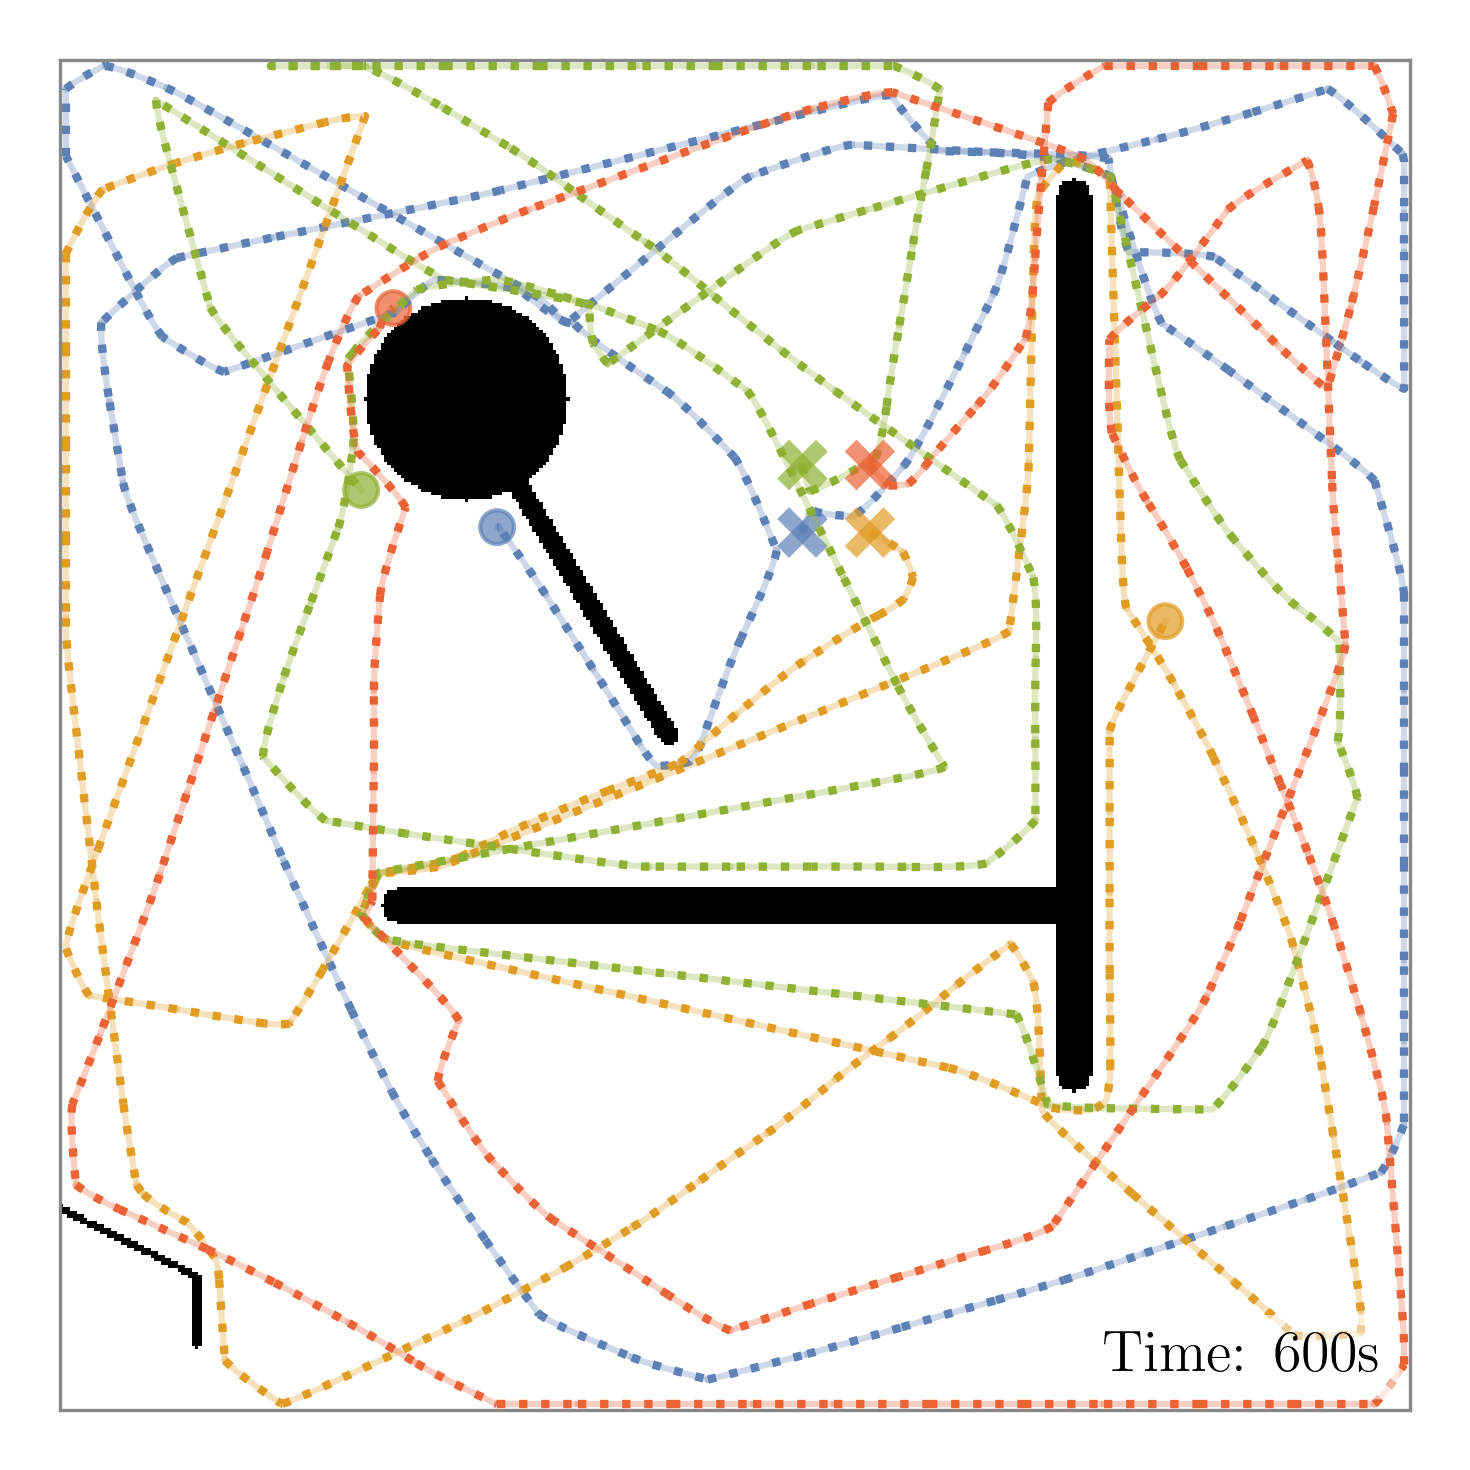
\includegraphics[width=\textwidth]{./figures/plots/paths/search:pathing-paths-(after-600s).png}
    \end{subfigure}
    \caption{Paths of four robots using the pure pathing algorithm. Dashed paths indicate full-time path-following. Crosses mark starting positions; circles indicate end positions.}
    \label{fig:pure-pathing-paths}
\end{figure}

The pure pathing algorithm also achieves full map coverage, with highly structured and efficient motion. A comparative analysis of all algorithms is presented in \cref{sec:results}.
